%%%%%%%%%%%%%%%%%%%%%%%%%%%%%%%%%%%%%%%%%%%%%%%%%%%%%%%%%%%%%%%%%%%%%%%%%%%%%%%%%
%%%%%                             SETTINGS                                   %%%%
%%%%%%%%%%%%%%%%%%%%%%%%%%%%%%%%%%%%%%%%%%%%%%%%%%%%%%%%%%%%%%%%%%%%%%%%%%%%%%%%%
\documentclass{article}

\usepackage{inputenc}
\usepackage{csquotes}
\usepackage[a4paper, total={6in, 9.2in}]{geometry}
\usepackage{hyperref}
\usepackage{dsfont}
\usepackage{amsmath,amssymb,dsfont}
\usepackage{graphicx}
\usepackage{indentfirst}
\usepackage{caption}
\usepackage{subcaption}
\usepackage{booktabs}
\usepackage{setspace}
\usepackage{indentfirst}
\usepackage[inline]{enumitem}
\usepackage{lscape}

\usepackage{tikz}
\usetikzlibrary{decorations.pathreplacing, positioning, arrows.meta}

\setlength{\parskip}{.5em}%

\usepackage[backend = biber,
		   style = authoryear,
		   maxnames = 5,
		   maxcitenames = 3,
		   doi = false,
		   eprint = false]{biblatex}
\addbibresource{../biblio.bib}

\newcommand{\aref}[1]{\hyperref[#1]{Appendix~\ref{#1}}}

\def\equationautorefname~#1\null{%
  equation~(#1)\null
}

%%%%%%%%%%%%%%%%%%%%%%%%%%%%%%%%%%%%%%%%%%%%%%%%%%%%%%%%%%%%%%%%%%%%%%%%%%%%%%%%%
%%%%%                                TITLE                                   %%%%
%%%%%%%%%%%%%%%%%%%%%%%%%%%%%%%%%%%%%%%%%%%%%%%%%%%%%%%%%%%%%%%%%%%%%%%%%%%%%%%%%

\title{Do Minimum Wages Increase Rents? 
	   Evidence from U.S. Zipcodes using High Frequency Data \thanks{We thank ...}}
\author{Gabriele Borg \and Diego Gentile Passaro \and Santiago Hermo
		\footnote{Borg: Department of Economics, Brown University (email: 
		\url{gabriele_borg@brown.edu}); 
		Gentile Passaro: Department of Economics, Brown University (email: 
		\url{diego_gentile_passaro@brown.edu}); 
		Hermo: Department of Economics, Brown University (email: 
		\url{santiago_hermo@brown.edu}).}
		}
\date{\today}


%%%%%%%%%%%%%%%%%%%%%%%%%%%%%%%%%%%%%%%%%%%%%%%%%%%%%%%%%%%%%%%%%%%%%%%%%%%%%%%%%
%%%%                              STRUCTURE                                  %%%%
%%%%%%%%%%%%%%%%%%%%%%%%%%%%%%%%%%%%%%%%%%%%%%%%%%%%%%%%%%%%%%%%%%%%%%%%%%%%%%%%%

\begin{document}

\maketitle

\begin{abstract}
    \noindent 
    In this paper, we estimate the effect of minimum wage policies on housing rental prices. 
    To do so, we construct a panel data set at the zipcode-month level using data from Zillow 
    and state and local minimum wage changes between 2010 to 2019. Our baseline empirical 
    approach assumes that, conditional on monthly date and zipcode fixed effects, 
    unobservable determinants of median rents are uncorrelated with past and future minimum 
    wage changes. Results indicate that increasing the minimum wage 10 percent is associated 
    with an increase of between 0.25 and 0.5 percent in median rents per square foot. We use 
    several alternative empirical approaches and construct falsification tests that support a 
    causal interpretation of this estimate. We show evidence that indicates the effect is 
    driven by zipcodes where minimum wage workers reside. Further heterogeneity analysis 
    indicates that the effect is larger in zipcodes with a high proportion of unemployed, 
    African-American, and low-income households.
\end{abstract}

\vspace{5mm}

\maketitle
\onehalfspacing

\clearpage

\section{Introduction}\label{sec:intro}
    %%%%%%%%%%%%%%%%%%%%%%%%%%%%%%%%%%%%%%%%%%%%%%%%%%%%%%%%%%%%%%%%%%%%%%%%%%%%%%%%%
%%%%%                            INTRODUCTION                                %%%%
%%%%%%%%%%%%%%%%%%%%%%%%%%%%%%%%%%%%%%%%%%%%%%%%%%%%%%%%%%%%%%%%%%%%%%%%%%%%%%%%%

In recent years, many US jurisdictions have introduced minimum wages (hereafter MW) above the 
federal level of \$7.25.\footnote{As of January 2020, there were 29 states that set a minimum 
	wage higher than the federal minimum, 52 counties that set a higher minimum wage than the 
	state, and 15 cities that set a higher minimum wage than the county.}
Despite prominent debates on recent MW policies both at the local and national level, ever since 
\textcite{card2000minimum} most research effort has been devoted to understanding the effects of MW on employment \parencite{neumark2006minimum, dube2010minimum, dube2016minimum}. This is not surprising, 
as employment effects are of first order importance to understand the welfare implications of MW 
changes on households. However, the \textit{place-based} nature of MW provisions make it natural to 
expect such policies to affect the welfare of households through markets other than the labor one. 
By far, the most prominent candidate to investigate is the housing market, and the channels through 
which it may fuel growing disparity in income and opportunities across the US. How much do local rents 
react to MW changes? Surprisingly, there is very little research estimating such effect,\footnote{To 
	our knowledge the only papers aiming at answering this question are 
	\textcite{yamagishi2019minimum} and \textcite{tidemann2018mw} Both papers found opposing results despite using the same year-county data. \textcite{yamagishi2019minimum} finds a small positive effect, while \textcite{tidemann2018mw} finds a small negative effect. \textcite{yamagishi2019minimum} 
	attributes this difference to different model specifications, and argues that with proper standard 
	errors clustering the results in \textcite{tidemann2018mw} are statistically insignificant. We 
	will soon explain the differences of this paper with those.} 
and virtually no research estimating the effects on local amenities.

A canonical version of the Alonso-Muth-Mills monocentric city  model with homogeneous agents 
predicts that wage increases should be fully capitalized by landlords, as workers end up paying 
higher rents in all locations.\footnote{See \textcite{brueckner1987structure} for a complete treatment 
	of this model.} 
However, we lack a clear empirical estimate of how big the pass-through from a MW change to 
rents is. This simple example illustrates how the welfare implications and incidence of MW changes
may very well depend on what happens to rents. Furthermore, if the pass-through to rents is high, 
we may also expect a response of local amenities through residential sorting. As recently emphasized
by \textcite{diamond2016determinants}, accounting for the welfare implications of amenities may be 
important.
 
In this paper, we use data at the zipcode-month level to assess the reduced form effects of 
MW changes on rents. Estimating empirically the pass-through from MW to rents is relevant both 
from a policy and theoretical perspective. As shown by \textcite{agarwal2019minimum}, if landlords 
know that their tenants have more disposable income, raising the rent will have two consequences. 
On one hand, it increases the landlords revenue conditional on receiving the rent payment. On the 
other hand, it increases the probability of tenants defaulting their payment.

Estimating the MW-rent pass-through is empirically challenging as it requires exogenous variation 
in the MW. It appears plausible that determinants of local level MW changes might correlate with 
geographical and time factors also affecting the housing market. To overcome this challenge, we 
follow \textcite{meer2016effects} and use several empirical approaches based on the panel data 
literature. Our main specification builds on a panel difference-in-differences (DiD) strategy 
that exploits the size and the fine timing of hundreds of MW changes across different US jurisdictions 
from 2010 to 2019. However, our approach differs from the usual DiD as we use insights from the 
event-study literature and from \textcite{arellano1991some}: we are able in this way to take into 
account both the potential dynamic effects of MW changes on rents and the persistence of the shock 
to the rental dynamics at the local level. MW changes are staggered across zipodes and dates, and 
this allows us to rely on within zipcode variation around MW changes to estimate the relevant pass-through by controlling for zipcode and time fixed effects. Since many zipcodes experience 
multiple MW changes, our specifications do not suffer from the underidentification problem arising 
when units are treated only once \parencite{BorusyakJaravel2017}.

Our baseline specification yields the true causal effect of MW changes on rents assuming that, 
within a zipcode, time-varying factors leading to MW changes are not related to unobservable 
determinants of the rental price dynamics. We provide several tests for the validity of our 
identification strategy: first, we test for differential pre-trends between treated and control 
units. We do this using the insight from \textcite{granger1969investigating}: we add leads of the 
MW changes and show that there are not anticipatory effects in treated zipcodes relative to 
untreated ones. Intuitively, if effects are being driven by some preexisting time-varying 
unobserved difference between treated and untreated zipcodes we should see that future MW changes 
have effect in the rental prices. Second, we check for the presence of unobservables affecting both 
rents and MW changes with proxies for local economic shocks as well as shocks to the housing market. 
Third, we allow for unobserved shocks to rent prices to be not iid by including a lagged dependent 
variable in our specification. Our results survive all of those tests. In addition, our identification 
strategy has the advantage of plausibly having more external validity than research based on a few 
case studies as it scrutinizes the dynamics of rental prices around hundreds of MW changes all over 
the US in a long period of time. In addition, we test the degree of sample bias by reweighting our 
data to match demographic characteristics of the average US zipcode. Our effects not only survive 
but are bigger and more precisely estimated. Finally, we make sure that our effects are not driven 
by changes in the composition of zipcodes appearing in our data through estimating our model in 
under both balanced and unbalanced panel data sets. 

Our results reveal a small yet robust impact of MW changes on rents. The \textit{static} 
difference-in-differences specification shows how a 1 percent increase in the MW leads to an average 
0.026 percent increase in the rental price per square foot. When expanding the model to account for 
\textit{dynamic} effects, we find a statistically significant impact in the first two months following 
a MW change: for the average zipcode a 10 percent increase in MW rents increase between 0.25\% and 
0.5\%. In an effort to understand who are the ``winners and losers", we perform an heterogeneity 
analysis of the estimated impact that reveals how results are driven by effects in zipcodes that are 
more likely to have minimum wagers as residents: those that have a highest share of unemployed, lower 
household income, and a larger share of African-American population. The pass-through for these 
zipcodes is around twice as large. Consistently, we show that zipcodes with very low probability of 
having minimum wage workers as residents exhibit no significant effects. On the other hand, we find 
that the effect is constant across zipcodes with different share of MW workers that work there.

Our approach has several differences with respect to previous research on the topic. Both 
\textcite{tidemann2018mw} and \textcite{yamagishi2019minimum} use Fair Markets Rents data which is 
available at the yearly level and aggregated at the geographical level of counties.\footnote{
	\textcite{yamagishi2019minimum} also uses data at the year-prefecture level for the 47 Japanese 
	prefectures.} 
An important advantage of our approach is that we use the exact timing of the MW change at the monthly 
level. When using variation arising from a yearly frequency some units are "partially treated" which 
will tend to understate the magnitude of the effect. Furthermore, some jurisdictions have MW changes 
on many subsequent years, making it challenging to estimate the dynamics around changes that are 
followed by changes in the immediate year. For example, if there is a change in two subsequent years, 
then the estimated effect of the change in the second year may be due too the effect of the current MW 
change or to the past MW change or both. We are able to show that raising the MW increases rents 
significantly only in the first couple of months after implementation.

An important difference is that we use data at the zipcode- instead of the county-level. As of 2019 
there were 3,142 counties and 39,295 meaningful zipcodes in the US.\footnote{We exclude military and 
unique business zipcodes as they are irrelevant for house prices.} We illustrate the importance of 
having smaller units of analysis with the following example. For a given county \textit{a}, suppose 
that (1) all low skill jobs are in one particular zipcode; and (2) low skill households prefer to live 
near their jobs. Further assume that, following a MW change, employment effects are near 
zero.\footnote{This is consistent with the findings of \textcite{card2000minimum} and 
	\textcite{cengiz2019effect}, among others.}
One should then expect demand for housing in the zipcode with the low skill jobs to increase and 
demand for housing in the rest of the zipcodes to go down. If we focus on the effects of the MW 
increase on the county we might even find that the rents go down, when in fact the rents in the 
zipcodes were the low skill jobs are located are increasing. Indeed, \textcite{tidemann2018mw} found 
that a \$1 increase in the MW decreases the yearly average of the monthly rent by 1.5 percentage 
points.\footnote{As pointed out by \textcite{tidemann2018mw}, the sign of this effect implies that 
	the labor demand for low skilled workers is elastic. This is at odds with the results from 
	\textcite{card2000minimum}, \textcite{cengiz2019effect}, and many others.}

% If we add amenities to the example, matters become much more complicated but if we allow for high 
% skill people to value amenities differently than low skill people (like in 
% \textcite{diamond2016determinants}), we may also expect to see residential resorting of high skill 
% people depending on where are the amenities located, whether the amenities respond endogenously to 
% the high-low skill composition of the zipcode, and depending on which are the zipcodes that the low 
% skilled workers are demanding less. This example, illustrates that as the spatial distribution of 
% jobs and amenities varies at the very local level, when tastes are heterogeneous by skill (or some 
% other dimension) focusing on a large geographic area may be misleading. 

A second advantage of having a more detailed geography is that we can also exploit MW changes at any 
jurisdictional level, effectively increasing the number of events used for identification. This is 
interesting because MW changes at different jurisdiction levels may have different local effects on 
rents.
% Intuitively, this is the case because, for example, out-of-state migration is in principle more 
% costly than out-of-county migration.  therefore, we expect more residential resorting within a state 
% and across counties when a county changes their local MW wage. Our data allows us to study the 
% heterogeneous effects of different MW changes.\footnote{In principle, our data allows us to answer 
% whether the effects of changes at the federal, state, county, and city/town level are different.} 

% we can use the census to compute the level of employment and the distribution of income in each %  
% zipcode, and check if we observe stronger effects on rents in places where there are more MW earners 
% or in places where there is more low skilled employment. 

A third difference of our approach is that by exploiting data at the zipcode monthly level we can go 
well beyond two-way county-year fixed-effect models. This is important because the dynamics of the 
rental market plausibly vary across zipcodes within a county following trends at the very local level 
\parencite{almagro2019location}. Our baseline specification has zipcode and monthly date fixed 
effects. Furthermore, in order to allow for heterogeneity in rental dynamics at the zipcode level we 
allow for zipcode-specific linear and quadratic terms. This in turn has two advantages. First, it 
makes our estimates more precise than the previously available ones. Second, and most importantly, it 
makes the required identification assumptions substantially more plausible. Given that the identifying 
variation comes from within-zipcodes, the determinants of these MW changes are unlikely to be related 
to the particular zipcode, and therefore, are less likely to be correlated to the unobservable 
determinants of rent dynamics there.

% A fourth important difference with past work, is that to the best of our knowledge, this is the 
% first study that estimates the effect of MW changes on amenities. As pointed out recently by 
% \textcite{diamond2016determinants, almagro2019location}, taking into account non-pecuniary  
% dimensions of the utility function can change substantively the welfare computations and the 
% incidence of policy relevant changes. We exploit the use of high frequency GPS data to build amenity 
% measures at the zipcode-month level and estimate the effect of MW changes on them. We hope that by 
% incorporating amenities into the picture we can give a more comprehensive assessment of the effects 
% of MW policies.

Beyond the contribution to the very recent literature on the effects of MW changes on rents, we 
contribute to several strands of the economic literature. First, we contribute to the literature 
studying the effects of minimum wages on the welfare of low skill households. However, instead of 
focusing on wages and employment \parencite[][among others]{dinardo1995labor, autor2016contribution, 
card2000minimum, neumark2006minimum, jardim2017minimum}, we contribute to this strand of literature 
by taking into account the effects on the housing market.

Second, our work relates to the literature that studies the location decision of agents either based 
on income \parencite{roback1982wages, kennan2011effect, desmet2013urban, perez2018city} or based on 
spatial rent and amenity differentials \parencite{diamond2016determinants, almagro2019location, 
couture2019income, bayer2004equilibrium}. We hope to contribute by adapting this framework to the 
case of the MW changes, so that we can rationalize through residential location sorting part of 
the observed reduce form effect on rents and amenities.

The rest of the paper is organized as follows. Initially, section \ref{sec:model} motivates the paper
with a simple model of the rental market. In section \ref{sec:data}, we present our data sources and 
show the characteristics of our estimating panel. In section \ref{sec:empirical_strategy}, we explain 
our empirical strategy and we discuss our identification assumptions. In section \ref{sec:results}, we 
present our main results. Section \ref{sec:discussion} discusses relevant policy implications, and 
section \ref{sec:conclusion} concludes.


\section{A simple model of the local rental market}\label{sec:model}
    %%%%%%%%%%%%%%%%%%%%%%%%%%%%%%%%%%%%%%%%%%%%%%%%%%%%%%%%%%%%%%%%%%%%%%%%%%%%%%%%%
%%%%%                                MODEL                                   %%%%
%%%%%%%%%%%%%%%%%%%%%%%%%%%%%%%%%%%%%%%%%%%%%%%%%%%%%%%%%%%%%%%%%%%%%%%%%%%%%%%%%

TO ADD




\section{Data and sample selection criteria}\label{sec:data}
	%%%%%%%%%%%%%%%%%%%%%%%%%%%%%%%%%%%%%%%%%%%%%%%%%%%%%%%%%%%%%%%%%%%%%%%%%%%%%%%%%
%%%%%                             DATA SAMPLE                                %%%%
%%%%%%%%%%%%%%%%%%%%%%%%%%%%%%%%%%%%%%%%%%%%%%%%%%%%%%%%%%%%%%%%%%%%%%%%%%%%%%%%%

Our main data is a panel at the US postal service zipcode-month level from January 2010 to December 
2019. This panel comes from five distinct sources.

First of all, our data contains MW changes at the federal, state, county, and city level.\footnote{
	Note that federal level MW changes still could induce meaningful variation as it is binding in 
	some zipcodes and not in others, so that identification does not come only from time series 
	variation. However, the last federal MW increase was in 2009 so changes used in our estimates come 
	from state, county, and city level.} 
Most of these changes come from \textcite{VaghulZipperer2016} and \textcite{CegnizEtAl2019}, but 
we updated this data for the years 2017, 2018, and 2019. For each zipcode we assume that the prevailing 
MW at a given month is the maximum between the required by the federal, state, county, and city levels. 
We only use MW changes that are binding, so only changes that actually change the maximum. In our 
baseline panel, we use 5,301 MW changes at the zipcode-month level. These changes are constructed out 
of 166 state level changes and 229 county and city level changes.

% In our baseline estimates we exclude county and city level changes because they might have different 
% effects on rents and amenities. We include prominent MW changes at those levels in robustness checks, 
% and in specifications that allow explicitly for heterogeneous effects at the different jurisdiction 
% levels.

Second, we use rent and house value data from properties listed in Zillow \parencite{zillow} in our 
sample period. Zillow is the leader online real estate and rental platform in the U.S., hosting more 
than 110 million homes and 170 million unique monthly users in 
2019.\footnote{\href{https://www.zillowgroup.com/facts-figures/}
	{\texttt{https://www.zillowgroup.com/facts-figures/}} (accessed on October 23rd, 2020).}  
Zillow provides the median rental and listing price (both total and per square foot) at which homes 
were listed on the platform. Time series are provided for different house types, and for different 
geographic aggregation level.\footnote{\href{https://www.zillow.com/research/data/}
	{https://www.zillow.com/research/data/} provides more information on the data shared by Zillow. 
	The availability of different time series changed over time, so not all series used for the 
	analysis might be still available to download.} 
We choose to focus on USPS zipcode level monthly time series so to capture the local behavior of the 
housing market. Clearly, even within a single zipcode, there could be great heterogeneity in terms of 
house sizes and types, making it more difficult to assess the impact of local intervention. In an 
effort to minimize price variation coming from houses' characteristics, such as the number of bedrooms, 
we focus our main analysis on the single family, condominium and cooperative homes (SFCC) series. 
This is by far the series with the largest number of non-missing zipcode, as it covers the most 
common U.S. rental house types. In 2018, roughly a third of the nation's 47.2 million rental units 
were single-family homes, while another 43 percent was made up from buildings with 5 or more units 
\parencite{JCHS2020}. We then select -- for all our analysis -- \textit{per square foot} 
variables: this allows us to reduce confonding variation based on supply-side factors such as land 
availability. A limitation in the use of Zillow data comes from the fact that we cannot observe the 
underlying number of houses listed for rent in a given month. Changes in the Zillow inventory 
therefore introduce additional variation in the reported median rental price.

In \autoref{tab:desc_stats}, we compare descriptive statistics for our data and for representative 
US aggregates from the 2010 Census and the 5 years 2008 ACS. Columns 1 and 2 report data for the 
whole universe of US zipcodes and for the top 100 US metropolitan areas respectively. In column 3 
we show the complete set of Zillow data. Finally, in column 4 we restrict our sample by balancing 
the panel keeping fixed the number of zipcodes only using zipcodes that have complete SFCC rental 
data (baseline sample). Focusing on our preferred series, Zillow provides information on rents for 
4,604 unique zipcodes accounting for 11.8 percent of the US zipcodes and 46.7 percent of the 2015 US population. 
The average median household annual income for those zipcodes is \$64,289, 22.5 percent higher than 
the same figure for the average US zipcode, but it is slightly lower than the figure for the average 
zipcode in the top 100 metropolitan areas. Zipcodes in the baseline sample are more populous and 
slightly higher income than the average US zipcode. Zillow is a real estate company and as such it 
is present in more dynamic rental markets. Those markets have a higher share of urban population, a 
higher share of college students, and a higher share of house for rent that the average US zipcode. 
For these reasons, and given that we will show that our effects are driven by the lower income 
zipcodes in our sample, we interpret our estimates as a lower bound for the true average treatment 
effect.

To ensure that our data correctly captures the price evolution of the US rental market, we compare 
Zillow's median rental price with 5 Small Area Fair Market Rents (SAFMRs) series for houses with 
different number of bedrooms (0, 1, 2, 3, and 4 or more) coming from the US Department of Housing and 
Urban Development (\citeyear{hud}). SAFMRs are calculated for zipcodes within metropolitan areas at a 
yearly level, and generally equal the 40th percentile of the rent distribution for that 
zipcode.\footnote{For more information on how SAFMRs are calculated, see page 41641 of the 
	\href{https://www.huduser.gov/portal/datasets/fmr/fmr2018/FY2018-FMR-Preamble.pdf}
	{Federal Register/Vol. 82, No. 169}} 
The yearly time series correlation between Zillow SFCC and all of the SAMFRs series is consistently 
above 90 percent. Single family houses, as well as condos and cooperative houses, are fairly loose 
categories and are therefore expected to vary in terms of the number of bedrooms they might have. For 
this reason, in \autoref{fig:trend_zillow_safmrwgt} we compare the Zillow SFCC series with a weighted 
combination of the different SAMFRs series.\footnote{To compute the weighted SAMFR series we proceed 
	as follows. First, we compute the national yearly average for both the Zillow SFCC and the 5 
	SAFMR series. Then, for each of the latter we compute the U.S. share of single family, condo, 
	and cooperative houses with that number of bedrooms using the \textit{American Housing Survey} 
	(AHS). To ensure comparability, we only use the estimated count for rental houses in this step. 
	(Additionally, AHS data is available only for years 2011, 2013, 2015, 2017, and 2019. We therefore 
	fill missing years with previous year's share.) Finally, we weight SAFMR series using the 
	aforementioned shares.} 
The Zillow rent data is always higher in levels. Part of this difference is intuitively related to the 
fact that Zillow reports median rent prices while SAFMRs are based on the 40th percentile of the rent 
distribution. The two series however show similar trends, confirming that Zillow rental series indeed 
captures the dynamics of the U.S. rental prices.

% As for the information on house values, Zillow has data on 10875 unique zipcode that correspond to 
% \%27.7 of the zipcodes and to \%78.9 of the 2015 population. The average median household annual 
% income for those zipcodes in 2015 was \$69556, which is \%17 higher than the same figure for all 
% the US zipcodes

\begin{table}[h!]
    \caption{Descriptive statistics and comparison with representative zipcodes}
    \centering
    \label{tab:desc_stats}    
    \begin{tabular}{l*{4}{c}}
\hline\hline
            &           t&            &            &            \\
            &        U.S.&  Full Panel&Listing Panel&  Rent Panel\\
\hline
zipcode     &       38893&       32281&        7699&        1305\\
(\%)        &           1&         .83&        .198&        .034\\
population  &    1.61e+08&    1.34e+08&    3.68e+07&     6648540\\
(\%)        &           1&        .831&        .228&        .041\\
housing units&    7.41e+07&    6.18e+07&    1.60e+07&     2811036\\
(\%)        &           1&        .834&        .216&        .038\\
median income&    52492.56&    53007.31&    63721.32&    66919.73\\
Houses for rent (\%)&        .294&        .259&        .304&         .38\\
Urban population (\%)&         .46&        .403&        .813&        .967\\
College Educated (\%)&        .313&        .304&        .389&        .441\\
Black population (\%)&        .086&        .076&        .095&        .165\\
Hispanic population (\%)&        .097&        .087&        .132&        .189\\
Pop. in poverty (\%)&        .155&        .145&        .126&        .135\\
Children 0-5 (\%)&        .185&        .188&        .193&        .195\\
Elders 65+ (\%)&        .151&        .155&        .141&        .114\\
Unemployed(\%)&         .09&        .087&        .088&        .094\\
Work in same County (\%)&        .702&        .683&        .722&        .758\\
MW events   &           .&       8.425&       3.703&       4.062\\
Salient MW events&           .&       4.487&       1.668&       1.608\\
Fed MW event&           .&        .322&           0&           0\\
State MW event&           .&       7.805&       3.232&       3.603\\
County MW Event&           .&        .165&        .277&         .12\\
Local MW Event&           .&        .132&        .194&        .339\\
medrentpricepsqft\_sfcc&           .&       1.372&           .&       1.213\\
medlistingpricepsqft\_sfcc&           .&     171.534&     161.503&           .\\
\hline\hline
\end{tabular}

   	\begin{minipage}{0.95\textwidth} \footnotesize
		\vspace{3mm} 
		\textit{Notes}: The table shows average values for the full sample (column 3), and the 
		restricted balanced samples, our baseline (column 4). In column 1 we report demographic 
		statistics for the universe of USPS zipcode we were able to map. In column 2 we report 
		demographic statistics for the top 100 CBSA. All demographic information comes from the 2010 
		Census and the 5-years 2008-2012 ACS.  
	\end{minipage}
\end{table}

\begin{figure}[!h]
    \centering
    \caption{National Time Series for Zillow and SAFMR data}
    \label{fig:trend_zillow_safmrwgt}
    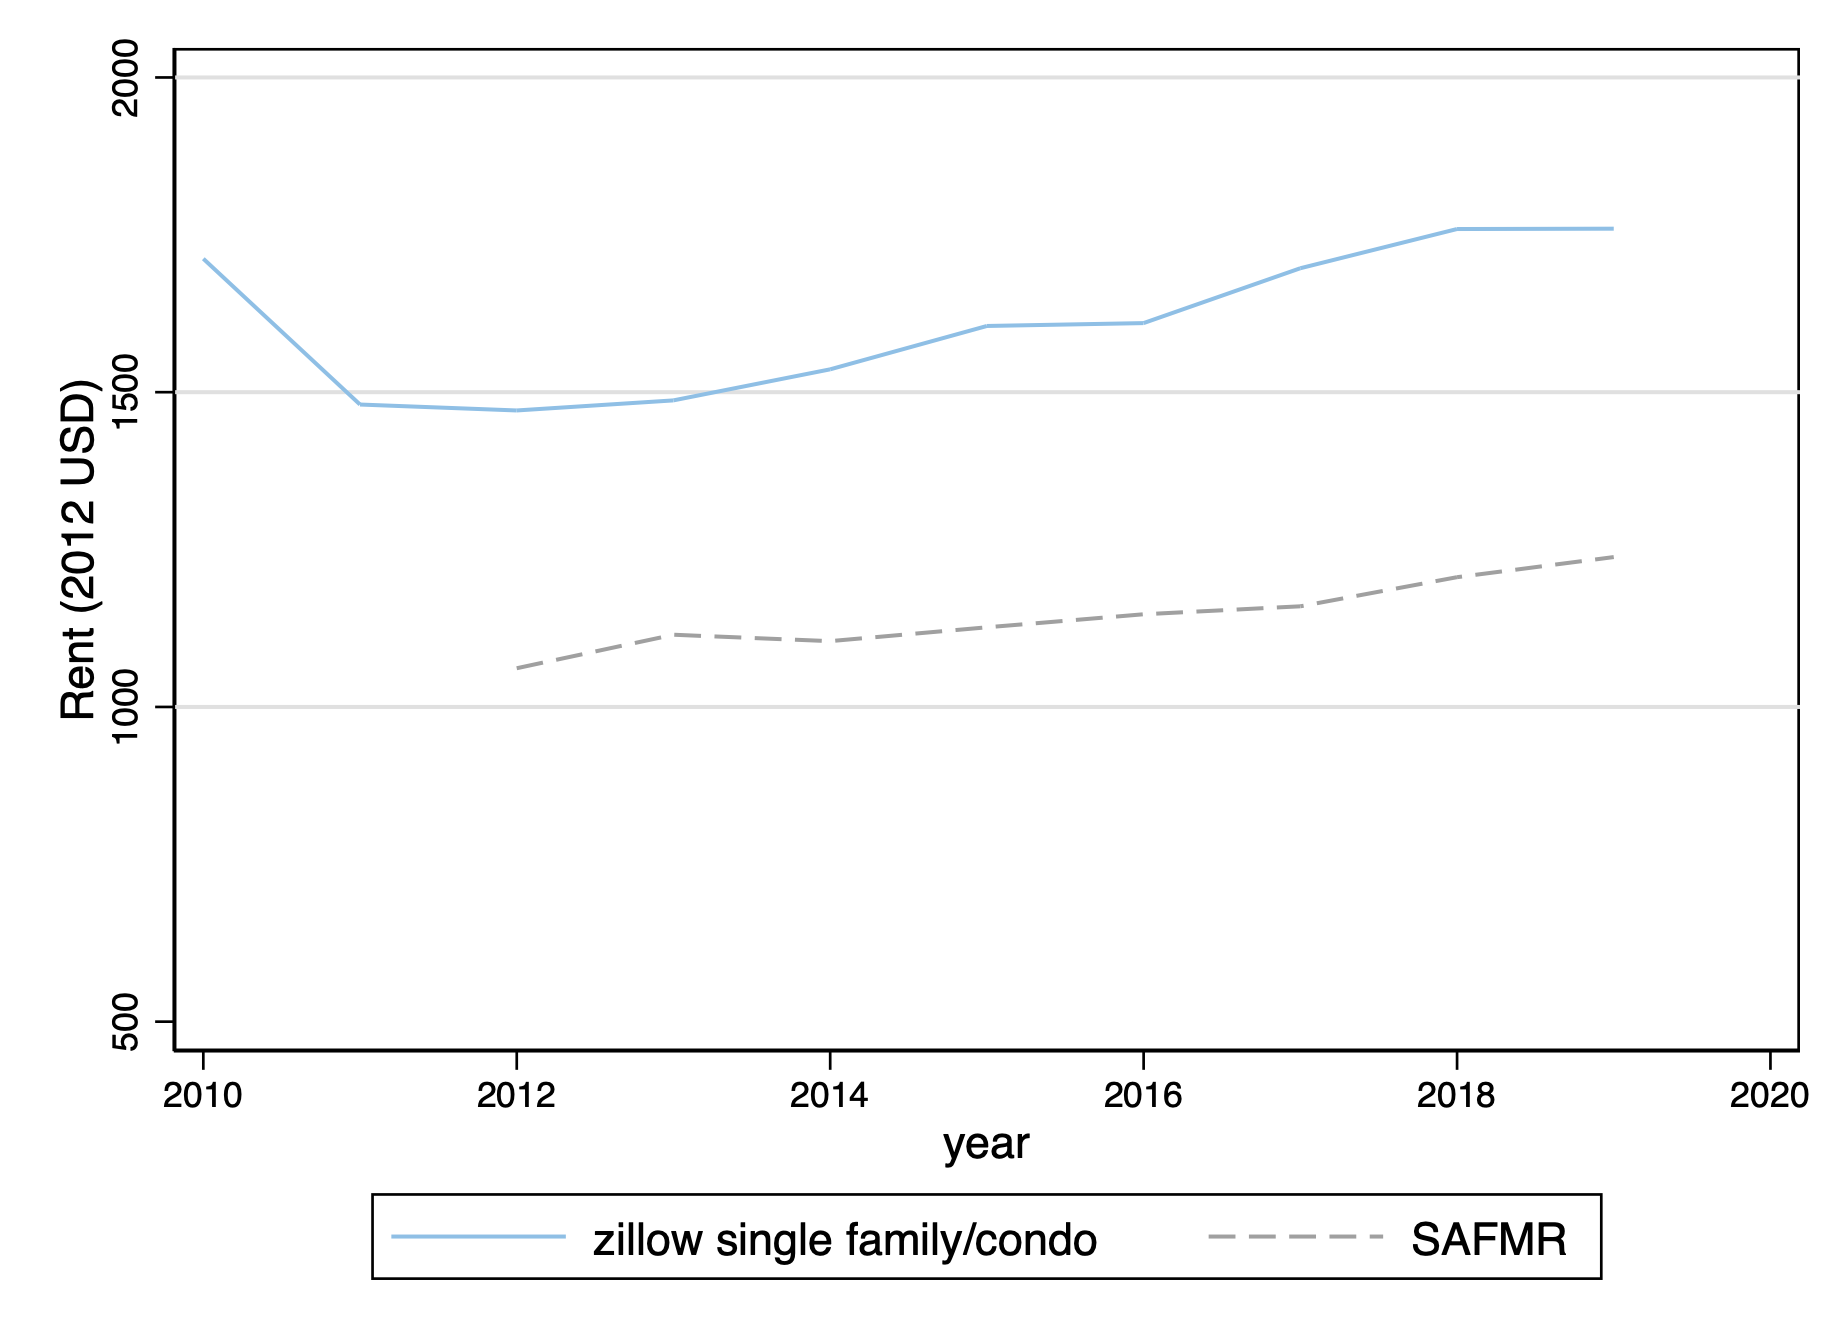
\includegraphics[width = 0.7\textwidth]{../../analysis/zillow_benchmark/output/trend_zillow_safmrwgt_zipcode_avg.png}
    \begin{minipage}{0.95\textwidth} \footnotesize
    	\vspace{3mm}
    	\textit{Notes:} The figure plots the monthly rent annual national average for the main Zillow 
    	series used in the analysis (SFCC) and a weighted combination of SAFMR series with different 
    	number of bedrooms. Weights are based on the US share of single family, condos and cooperative 
    	houses with given number of bedrooms as recorded in the AHS.    
    \end{minipage}
\end{figure}

Third, we add socio-demographic information to each zipcode in our sample using the 2010 Census and 
the 5-years 2008-2012 ACS. The data is originally obtained at the Census tract level and mapped into 
USPS zipcodes using HUD crosswalks.\footnote{Crosswalks are obtained from
	 \url{https://www.huduser.gov/portal/datasets/usps_crosswalk.html}} 
We assign to each zipcode the following characteristics: number of inhabitants, the number of houses, 
the median income, the number of black inhabitants, the number of unemployed, and the number of 
college students. We use this information to classify zipcodes into, for example, high or low median 
income to then perform heterogeneity analysis. In addition, given that zipcodes can cross county 
borders, we use the census data and geographic codes to map each zipcode to a county by assigning it 
to the one with the highest share of houses from that zipcode. We also map each zipcode to a 
metropolitan statistical area or a rural town analogously. We use this information to assign the 
prevailing MW to each zipcode.

% Fourth, to proxy for the quality of amenities at each location, we construct zipcode-month level 
% measures from GPS location point-of-interest data by SafeGraph\parencite{safegraph}. We define several 
% amenity measures. For our first measure, we follow closely \textcite{couture2019income} and construct 
% an index for the quality of restaurants available at each zipcode-month. This index is defined as the 
% average of the propensity of high-income individuals to visit a restaurant in a given zipcode 
% controlling for their distance to the establishments. In order to classify a visitor as high-income we 
% use the census tract location of the visitor. Our second measure is the same as the first but for the 
% quality of the visitors of open public spaces in each zipcode-month. For our third measure, we use the 
% point-of-interest data to count the number of restaurants, coffee shops, bars, and gyms per inhabitant 
% of a zipcode-month. 

Fourth, to proxy for local economic activity we collect data from the Quarterly Census of Employment 
and Wages (QCEW) at the county-quarter and county-month level for each industry and level of 
government.\footnote{The QCEW covers the following industries: goods-producing; natural resources and 
	mining; construction; manufacturing; service-providing; trade, transportation and utilities; 
	information; financial activities; professional and business services; education and health 
	services; leisure and hospitality. The QCEW additionally provides employment data for federal, 
	state, and local government.} 
For each county-quarter-industry cell we observe the number of establishments and the average weekly 
wage. For each county-month-industry cell we additionally observe the number of employed people. We 
merge this data onto our zipcode-month panel based on county and quarterly date.

We add data from the \textit{Building Permit Survey} (BPS) at the county-month level to account for 
time-varying shocks in the housing market. The BPS provides building permit statistics on new 
privately-owned residential construction disaggregated by house type. Lacking information on condos 
and cooperative houses, we only add the number of new units and the permits valuation for single 
family houses to each zipcode-month observation based on the county and month they belong.

Finally, we use data from the 2017 Longitudinal Employer-Household Dynamics Origin-Destination 
Employment Statistics (LODES) to proxy for MW workers' residence and workplace location. The LODES 
data sets provide block-level information on jobs and are organized in 3 groups: residence area 
characteristics (RAC), with information about characteristics of jobs for various types of workers 
(e.g. number of jobs in different sectors, number of job for workers under 30 years old, etc.); 
workplace area characteristics (WAC) that provide the same information as RAC files but aggregated 
with respect to workplace location; and a origin-destination matrix mapping jobs from residence to 
workplace locations. We use RAC and WAC datasets to ``locate" workers likely to be MW by looking at 
the state-level distribution of such type of workers: we build, for each zipcode in the sample, the 
share (out of the state total) of workers under 30 years old earning less than $\$1251$ that either 
\textit{live} or \textit{work} there. 


\section{Empirical strategy and identification}\label{sec:empirical_strategy}
    %%%%%%%%%%%%%%%%%%%%%%%%%%%%%%%%%%%%%%%%%%%%%%%%%%%%%%%%%%%%%%%%%%%%%%%%%%%%%%%%%
%%%%%                         EMPIRICAL STRATEGY                             %%%%
%%%%%%%%%%%%%%%%%%%%%%%%%%%%%%%%%%%%%%%%%%%%%%%%%%%%%%%%%%%%%%%%%%%%%%%%%%%%%%%%%

In this section, we present the empirical strategy adopted to study the effect of MW on rents, and 
we discuss the assumptions needed for identification. We begin with a panel DiD model and we build 
on that following \textcite{meer2016effects}. This allows us to estimate the full dynamics of rents 
around MW changes under various identifying assumptions. Our dynamic specifications are distinct 
from the usual DiD and event-study ones \parencite{BorusyakJaravel2017, abraham2018} for two main 
reasons: first, our models allow for the use of variation coming from more than one MW change per 
geographic unit and from geographic units that never experience a MW change. This is desirable 
because we both avoid under-identification issues with the two-way fixed effects and because we 
use never-treated zipcodes as control units. Secondly, our specifications not only exploit the 
timing of a MW change for identification but also its intensity.
    
% Whereas this shows a statistically significant results, one may worry about pre-trends that 
% confound the effect. To account for this, in the dynamic model we add leads and lags of this 
% variable, which allows us to formally test the hypothesis of pre-trends.


%%%%%%%%%%%%%%%%%%%%%%%%%%%%%%%%%%%%%%%%%%%%%%%%%%%%%%%%%%%%%%%%%%%%%%%%%%%%%%%%%
\subsection{Baseline Specifications}
Consider the following panel difference-in-differences model relating rents and the minimum wage:

\begin{equation}\label{eq:did_lev}
    y_{it} = \alpha_i + \alpha_t + \gamma_i t + \beta \underline{w}_{it} + \epsilon_{it}
\end{equation}
    
where $y_{it}$ is the log rent per square foot for the Zillow SFCC series, $\underline{w}$ is the 
log of the minimum wage, $\alpha_i$ is a zipcode fixed effect, $\alpha_t$ is a time fixed effect, 
and $\gamma_i$ is a zipcode-specific linear trend.\footnote{We add a zipcode-specific linear trend 
	to allow for heterogeneity in the time path of zipcodes \parencite{angrist2008mostly}. In the 
	next section we additionally present results from models without zipcode-specific linear trends 
	as well as with zipcode-specific quadratic trends.} 
We then re-write \autoref{eq:did_lev} in first differences:
    
\begin{equation}\label{eq:did}
        \Delta y_{it} = \theta_t + \gamma_i + \beta \Delta \underline{w}_{it} + \Delta \epsilon_{it}
\end{equation}

We reference this model as \textit{static DiD}. We spell out the model in first differences because 
we believe that the unobserved shocks to rental prices are likely to be persistent over time. Both 
the first differences and the level models are consistent under similar assumption but the first 
difference model is more efficient if the shocks are serially correlated \parencite{wooldridge2010}.

Identification comes from assuming that within a zipcode the change in the level of the logarithm 
of the minimum wage is mean independent of the change in the unobserved shock $\Delta \epsilon_{it}$ 
conditional on the time fixed effects and the zipcode-specific linear trend. This implies that if 
the true effect is a one-time level change, then $\beta$ has a causal interpretation and it can be 
seen as the elasticity of the rent per square foot to the MW.
    
One potential concern with the static DiD model, is that, despite controlling for a zipcode-specific 
linear trend, preexisting time-paths of rents per square foot might be different in zipcodes that 
had a MW change relative to zipcodes that did not experienced a change. To assess if that is the 
case, one can extend the model to include leads of $\Delta \underline{w}_{it}$. In addition, one 
may be believe that the effect of MW changes on rents is not a one time discrete level jump but that 
it also affects the growth rate of rental prices. In such cases the estimated coefficient $\beta$ 
from \autoref{eq:did} might only have limited relevance in evaluating the policy of interest 
\parencite{callaway2019difference}. To allow for dynamics in the effects, we extend the model to 
also include lags of $\Delta \underline{w}_{it}$. The \textit{dynamic} model is

\begin{equation}\label{eq:leads_lags}
    \Delta y_{it} = \theta_t + \gamma_i + \sum_{r=-s}^{s}\beta_r \Delta \underline{w}_{i(t-r)} 
    				+ \Delta \epsilon_{it} \ ,
\end{equation}
where $s$ is the number of months of a symmetric window around the MW change. Note that this 
dynamic DiD model still allows for treatment and control groups to have different averages, even though 
it now requires a more stringent identification: 
\[E \left[ \Delta \epsilon_{it} \Delta \underline{w}_{it-r} \big| \theta_{t}, \gamma_{i} \right] = 0
	\ \ \forall r\in\{-s, ..., -1, 0, 1, ..., s\} \ . \] 
In this context, a violation of the identification assumption would require a change in MW to be 
systematically correlated with unobserved shocks to treated zipcode relative to untreated ones. 
Importantly, this model allows us to test whether $\beta_{-s} = \beta_{-s+1} = ... = \beta_{-1} = 0$, 
the well known pre-trends test, to establish whether there are significant rent responses preceding 
a change in MW. Under the assumption of no pre-trends, we can gain efficiency through estimating a 
model only with distributed lags as follows:

\begin{equation}\label{eq:lags}
        \Delta y_{it} = \theta_t + \gamma_i 
        		+ \sum_{r=0}^{s}\beta_r \Delta \underline{w}_{i(t-r)} 
        		+ \Delta \epsilon_{it} \ .
\end{equation}

This model allows us to estimate the dynamics of the logarithm of the rent per square foot around 
changes in the MW and we can recover the elasticity of rents to MW by summing $\beta_0$ to 
$\beta_{s}$. We present results from this model in the results section. In past settings using 
yearly data \parencite{tidemann2018mw,yamagishi2019minimum}, MW changes are so common in a given 
geographic area relative to the timespan of the data that it is very hard to credibly estimate the 
lags. Intuitively, this is the case because it is hard to distinguish which variation of the rental 
price is due to the current MW change or to a preceding one. In our estimates that concern is not 
justified, as given that we have month to month variation, we use short windows (5 months) in which 
there is no overlap in MW changes within a zipcode. The absence of pre-trends does not exhaust the 
potential threats to identification. Effects could still be driven by contemporaneous shocks 
systematically affecting both changes in rents and MW within a zipcode. To ease those concerns, we 
directly control for several county-level time-varying proxies of the health of the local labor and 
housing markets.\footnote{This amounts to adding a vector $\Delta X_{ct}$ on the right-hand side of 
	our models, where $c$ indexes counties, and we map zipcodes to a single county as explained in 
	\autoref{sec:data}.} 
As mentioned in \autoref{sec:data}, part of the variation in the median rental price come from 
unobserved changes in the Zillow inventory for a given zipcode through time. This may pose a threat 
to identification...\textbf{TO FINISH}

Finally, in our appendix, we consider a dynamic panel specification to allow for full dynamics on 
the rental prices. The model then becomes

\begin{equation}\label{eq:ab_panel}
        \Delta y_{it} = \Delta y_{i(t-1)} + \theta_t + \gamma_i 
        		+ \sum_{r=0}^{s}\beta_r \Delta \underline{w}_{i(t-r)} 
        		+ \Delta \epsilon_{it} \ .
\end{equation}

However, by construction we now have that $\Delta y_{i(t-1)}$ is necessarily correlated with 
$\Delta \epsilon_{it}$. To address that, we take two separate approaches. First, we follow 
\textcite{arellano1991some} and, as it is customary in the literature, we instrument $\Delta 
y_{i(t-1)}$ with $\Delta y_{i(t-2)}$. Second, we follow \textcite{meer2016effects} and instrument 
$\Delta y_{i(t-1)}$ with an off-window lag of the change in the logarithm of the MW. In particular, 
as most of our models have a window $s=5$, we use as an instrument $\Delta \underline{w}_{i(t-6)}$. 
Intuitively, if there is an effect of MW changes to rents past MW changes should predict future 
rents and past MW changes should not be correlated with contemporaneous unobserved determinants 
of rents once we take into account the dynamic effect of MW on rents. 


%%%%%%%%%%%%%%%%%%%%%%%%%%%%%%%%%%%%%%%%%%%%%%%%%%%%%%%%%%%%%%%%%%%%%%%%%%%%%%%%%
\subsection{Heterogeneity by Zipcode Characteristics }

In order to allow for heterogeneous effects based on zipcode characteristics, and to make sure 
that our effects are driven by the zipcodes that are expected to have more MW earners, we extend the 
baseline panel difference-in-differences model defined in \autoref{eq:did} by interacting the local 
MW change with zipcode level characteristics. To minimize the possibility of any characteristic 
being endogenous to MW changes, we use use socio-demographic data that predate our panel. We take 
them from the 2010 Census and the 5-years 2008-2012 ACS. Then, the model we take to the data becomes

\begin{equation}\label{eq:diff_main_hetero} 
    \Delta y_{it} = \theta_t + \gamma_i 
    		+ \sum_{q = 1}^4 \beta_q \mathds{1}\{i \in q\} \Delta \underline{w}_{it} 
    		+ \Delta \epsilon_{it} \ ,
\end{equation}
where $q$ identifies quartiles of some zipcode level characteristic, and $\mathds{1}\{ \cdot \}$ is 
the indicator function. We report results for these models in \autoref{sec:heter}.

\section{Results}\label{sec:results}
    %%%%%%%%%%%%%%%%%%%%%%%%%%%%%%%%%%%%%%%%%%%%%%%%%%%%%%%%%%%%%%%%%%%%%%%%%%%%%%%%%
%%%%%                                RESULTS                                 %%%%
%%%%%%%%%%%%%%%%%%%%%%%%%%%%%%%%%%%%%%%%%%%%%%%%%%%%%%%%%%%%%%%%%%%%%%%%%%%%%%%%%

In this section we present our main results. In all cases standard errors are clustered at the 
state level so to match the main source of variation of the MW changes. We initially show how the 
estimated elasticity of rents to MW is approximately 0.025 when adopting the \textit{static DiD} 
model. We then present estimates for the \textit{dynamic} models that highlight both the absence 
of pre-trends, and the presence of a 2-months dynamic effect: the cumulative impact of a 10 \% MW 
change is estimated to be between 0.5 and 0.6 \% over the course of the 5 months after the policy 
change.

In \autoref{sec:sample_rest} we assess to what extent our results are representative of the true 
underlying Average Treatment Effect in two ways. First, since Zillow is present in relatively more 
dynamic markets than the average U.S. zipcode, we reweight observations so as to match population 
demographics for the top 100 CBSA. We show that the estimated impact slightly increases to 0.035 
\% indicating how our estimates can be seen as a lower bound. Second, we expand the panel used 
for the estimation by including zipcodes ``entering" after 2010. We control for changes in zipcode 
composition by contolling for \textit{entry cohort} $\times$ \textit{year-month} and we show how 
results are robust. We subsequently check for the presence of unobserved time-varying factors 
systematically affecting changes in MW and rents that may confound our estimates. We progressively 
include controls for the local economy, the labor and the housing market and we show how results 
do not change.

After establishing the robustness of our results, we then investigate how the incidence of the 
effect may vary across zipcodes. We use LODES data to proxy for MW workers residence and workplace 
location to show how effects disproportionately affect those zipcode that are more likely to have 
MW worker residents. We additionally estimate the heterogeneous impact of MW changes across the 
distribution of several census-based demographics. We show how effects are disproportionately 
concentrated in poorer, less-educated, and more African American zipcodes.


%%%%%%%%%%%%%%%%%%%%%%%%%%%%%%%%%%%%%%%%%%%%%%%%%%%%%%%%%%%%%%%%%%%%%%%%%%%%%%%%%
\subsection{Baseline Results}\label{sec:baseline_results}

In \autoref{tab:did_main}, we present results from the model defined in \autoref{eq:did}. In 
column 1, we show the classic two-way fixed effects (i.e. zipcode and year-month). To alleviate 
the concern that treated and untreated zipcodes could be on different time paths, in column 2 
(our baseline static DiD specification) we introduce linear time trends at the zipcode level. 
Finally, in column 3, we relax the linearity assumption on the zipcode-specific trends and allow 
for a quadratic time path for each zipcode. The estimated coefficients for MW changes are stable 
and significant across all specifications and indicate that a 10 percent increase in MW leads to 
a 0.26 percent increase in rent.

\begin{table}[h!]
    \caption{Results from Difference-in-Differences model}
    \label{tab:did_main}
    \centering
    {
\def\sym#1{\ifmmode^{#1}\else\(^{#1}\)\fi}
\begin{tabular}{l*{3}{c}}
\hline\hline
          &\multicolumn{1}{c}{(1)}&\multicolumn{1}{c}{(2)}&\multicolumn{1}{c}{(3)}\\
          &\multicolumn{1}{c}{D.ln\_med\_rent\_psqft}&\multicolumn{1}{c}{D.ln\_med\_rent\_psqft}&\multicolumn{1}{c}{D.ln\_med\_rent\_psqft}\\
\hline
D.ln\_mw   &   0.0257\sym{*}  &   0.0253\sym{**} &   0.0250\sym{**} \\
          & (0.0128)         & (0.0121)         & (0.0117)         \\
\hline
Zipcode-specifc linear trend&       No         &      Yes         &      Yes         \\
Zipcode-specific linear and square trend&       No         &       No         &      Yes         \\
R-squared &                  &                  &                  \\
Observations&    0.022         &    0.023         &    0.026         \\
N         &   113363         &   113363         &   113363         \\
\hline\hline
\end{tabular}
}

    \begin{minipage}{0.95\textwidth} \footnotesize
		\vspace{3mm} 
		\textit{Notes}: The table reports coefficients from versions of \autoref{eq:did} estimated 
		on the balanced panel of zipcode-months that contains SFCC rental price. Column (1) does not 
		include a zipcode-specific linear trend and results correspond to a two-way fixed effects 
		difference-in-differences. Column (2) includes zipcode-specific linear trends, and column (3) 
		allows for zipcode specific quadratic trends. Standard errors clustered at the state level. 
		*** $p < 0.01$, ** $p < 0.05$, * $p < 0.1$.
	\end{minipage}
\end{table}

In order to test for the presence of pre-trends in rents that may invalidate the causal 
interpretation of our results, we estimate the model with leads and lags of the MW changes defined 
in \autoref{eq:leads_lags}. We display the results in \autoref{tab:dynamic_lags_leads_main} and, 
again, present the results allowing progressively for more flexible zipcode level rental price 
heterogeneity over time.

\begin{table}[h!]
    \caption{Results from Difference-in-Differences model with leads and lags}
    \label{tab:dynamic_lags_leads_main}
    \centering
    {
\def\sym#1{\ifmmode^{#1}\else\(^{#1}\)\fi}
\begin{tabular}{l*{5}{c}}
\hline\hline
          &\multicolumn{1}{c}{(1)}         &\multicolumn{1}{c}{(2)}         &\multicolumn{1}{c}{(3)}         &\multicolumn{1}{c}{(4)}         &\multicolumn{1}{c}{(5)}         \\
\hline
$\Delta \ln \underline{w}_{ic,t-5}$&  -0.0148         &  -0.0144         &  -0.0144         &  -0.0146         &  -0.0144         \\
          & (0.0090)         & (0.0089)         & (0.0089)         & (0.0090)         & (0.0089)         \\
[1em]
$\Delta \ln \underline{w}_{ic,t-4}$&  -0.0024         &  -0.0019         &  -0.0020         &  -0.0022         &  -0.0019         \\
          & (0.0116)         & (0.0116)         & (0.0115)         & (0.0116)         & (0.0115)         \\
[1em]
$\Delta \ln \underline{w}_{ic,t-3}$&   0.0011         &   0.0005         &   0.0007         &   0.0004         &  -0.0002         \\
          & (0.0092)         & (0.0094)         & (0.0092)         & (0.0091)         & (0.0092)         \\
[1em]
$\Delta \ln \underline{w}_{ic,t-2}$&   0.0060         &   0.0063         &   0.0062         &   0.0060         &   0.0064         \\
          & (0.0116)         & (0.0118)         & (0.0116)         & (0.0115)         & (0.0117)         \\
[1em]
$\Delta \ln \underline{w}_{ic,t-1}$&  -0.0002         &  -0.0004         &  -0.0005         &   0.0000         &  -0.0005         \\
          & (0.0123)         & (0.0123)         & (0.0124)         & (0.0122)         & (0.0123)         \\
[1em]
$\Delta \ln \underline{w}_{ic,t}$&   0.0271\sym{**} &   0.0257\sym{**} &   0.0259\sym{**} &   0.0269\sym{**} &   0.0259\sym{**} \\
          & (0.0126)         & (0.0123)         & (0.0124)         & (0.0126)         & (0.0124)         \\
[1em]
$\Delta \ln \underline{w}_{ic,t+1}$&   0.0136\sym{*}  &   0.0146\sym{**} &   0.0142\sym{*}  &   0.0135\sym{*}  &   0.0146\sym{*}  \\
          & (0.0072)         & (0.0072)         & (0.0072)         & (0.0072)         & (0.0072)         \\
[1em]
$\Delta \ln \underline{w}_{ic,t+2}$&  -0.0070         &  -0.0066         &  -0.0064         &  -0.0068         &  -0.0064         \\
          & (0.0133)         & (0.0133)         & (0.0132)         & (0.0133)         & (0.0132)         \\
[1em]
$\Delta \ln \underline{w}_{ic,t+3}$&   0.0036         &   0.0045         &   0.0047         &   0.0031         &   0.0040         \\
          & (0.0081)         & (0.0078)         & (0.0078)         & (0.0079)         & (0.0077)         \\
[1em]
$\Delta \ln \underline{w}_{ic,t+4}$&   0.0108         &   0.0093         &   0.0104         &   0.0107         &   0.0096         \\
          & (0.0069)         & (0.0066)         & (0.0064)         & (0.0069)         & (0.0065)         \\
[1em]
$\Delta \ln \underline{w}_{ic,t+5}$&   0.0086         &   0.0095         &   0.0099         &   0.0088         &   0.0099         \\
          & (0.0069)         & (0.0065)         & (0.0065)         & (0.0067)         & (0.0065)         \\
\hline
\vspace{-2mm}&                  &                  &                  &                  &                  \\
Cumulative effect&    0.057         &0.057\sym{*}         &0.059\sym{*}         &    0.056         &0.058\sym{*}         \\
          &  (0.035)         &  (0.034)         &  (0.034)         &  (0.034)         &  (0.034)         \\
\hline    &                  &                  &                  &                  &                  \\
P-value no pretrends&    0.568         &    0.612         &    0.599         &    0.594         &    0.629         \\
Wage controls&       No         &      Yes         &       No         &       No         &      Yes         \\
Employment controls&       No         &       No         &      Yes         &       No         &      Yes         \\
Establishment-count controls&       No         &       No         &       No         &      Yes         &      Yes         \\
R-squared &    0.022         &    0.022         &    0.022         &    0.022         &    0.022         \\
Observations&  106,446         &  105,463         &  105,463         &  106,160         &  105,463         \\
\hline\hline
\end{tabular}
}

    \begin{minipage}{0.95\textwidth} \footnotesize
		\vspace{3mm} 
		\textit{Notes}: The table reports coefficients from versions of \autoref{eq:leads_lags} 
		estimated on the balanced panel of zipcode-months that contains SFCC rental price. Column 
		(1) does not include a zipcode-specific linear trend and results correspond to a two-way fixed-effects difference-in-differences. Column (2) includes zipcode-specific linear trends, 
		and column (3) allows for zipcode specific quadratic trends. Standard errors clustered at 
		the state level. *** $p < 0.01$, ** $p < 0.05$, * $p < 0.1$.
	\end{minipage}
\end{table}

Consistent with a causal interpretation of our results, future MW changes do not have an effect on 
rent prices. This suggests how there are no pre-treatment differentials in the evolution of rental 
prices between treated and untreated zipcodes. \autoref{tab:dynamic_lags_leads_main} additionally 
reports the results of an F-test for all leads to be jointly equal to zero. We comfortably fail to 
reject that hypothesis in all cases. On the other hand, we detect a significant effect on rents at 
the period of the MW change. Specifically, we estimate that rents increase by around 0.27 percent 
following a $10$ percent raise in the MW (column 2), and the effect is largely unchanged both by the 
exclusion of linear trends (column 1) and by the inclusion of more flexible zipcode quadratic level 
trends (column 3).

A second important result shown by \autoref{tab:dynamic_lags_leads_main} is the presence of a mild 
persistence of the effect of MW changes on rents. After a 10 percent change in the MW, rents tend to 
increase by $0.13$ percent in the month \textit{after} the change, while the impact appears to vanish 
after the first two periods. In column 3 the estimated coefficients in $t+1$ loses statistical 
significance being slightly lower, but the point estimate remains larger than any of the following 
post-treatment periods. The results shown implies that - when allowing for dynamic effects of MW 
changes on rents - the cumulative impact is even larger than the one estimated by the static DiD 
model. Over the course of a semester, a $10$ percent raise in the MW translates to between $0.5$ 
and $0.6$ percent increase in the rental price.

\begin{figure}
    \caption{Estimated Impact of changes in MW on changes in Rents for Different Specifications}
    \label{fig:fd_models_main}
    \centering
    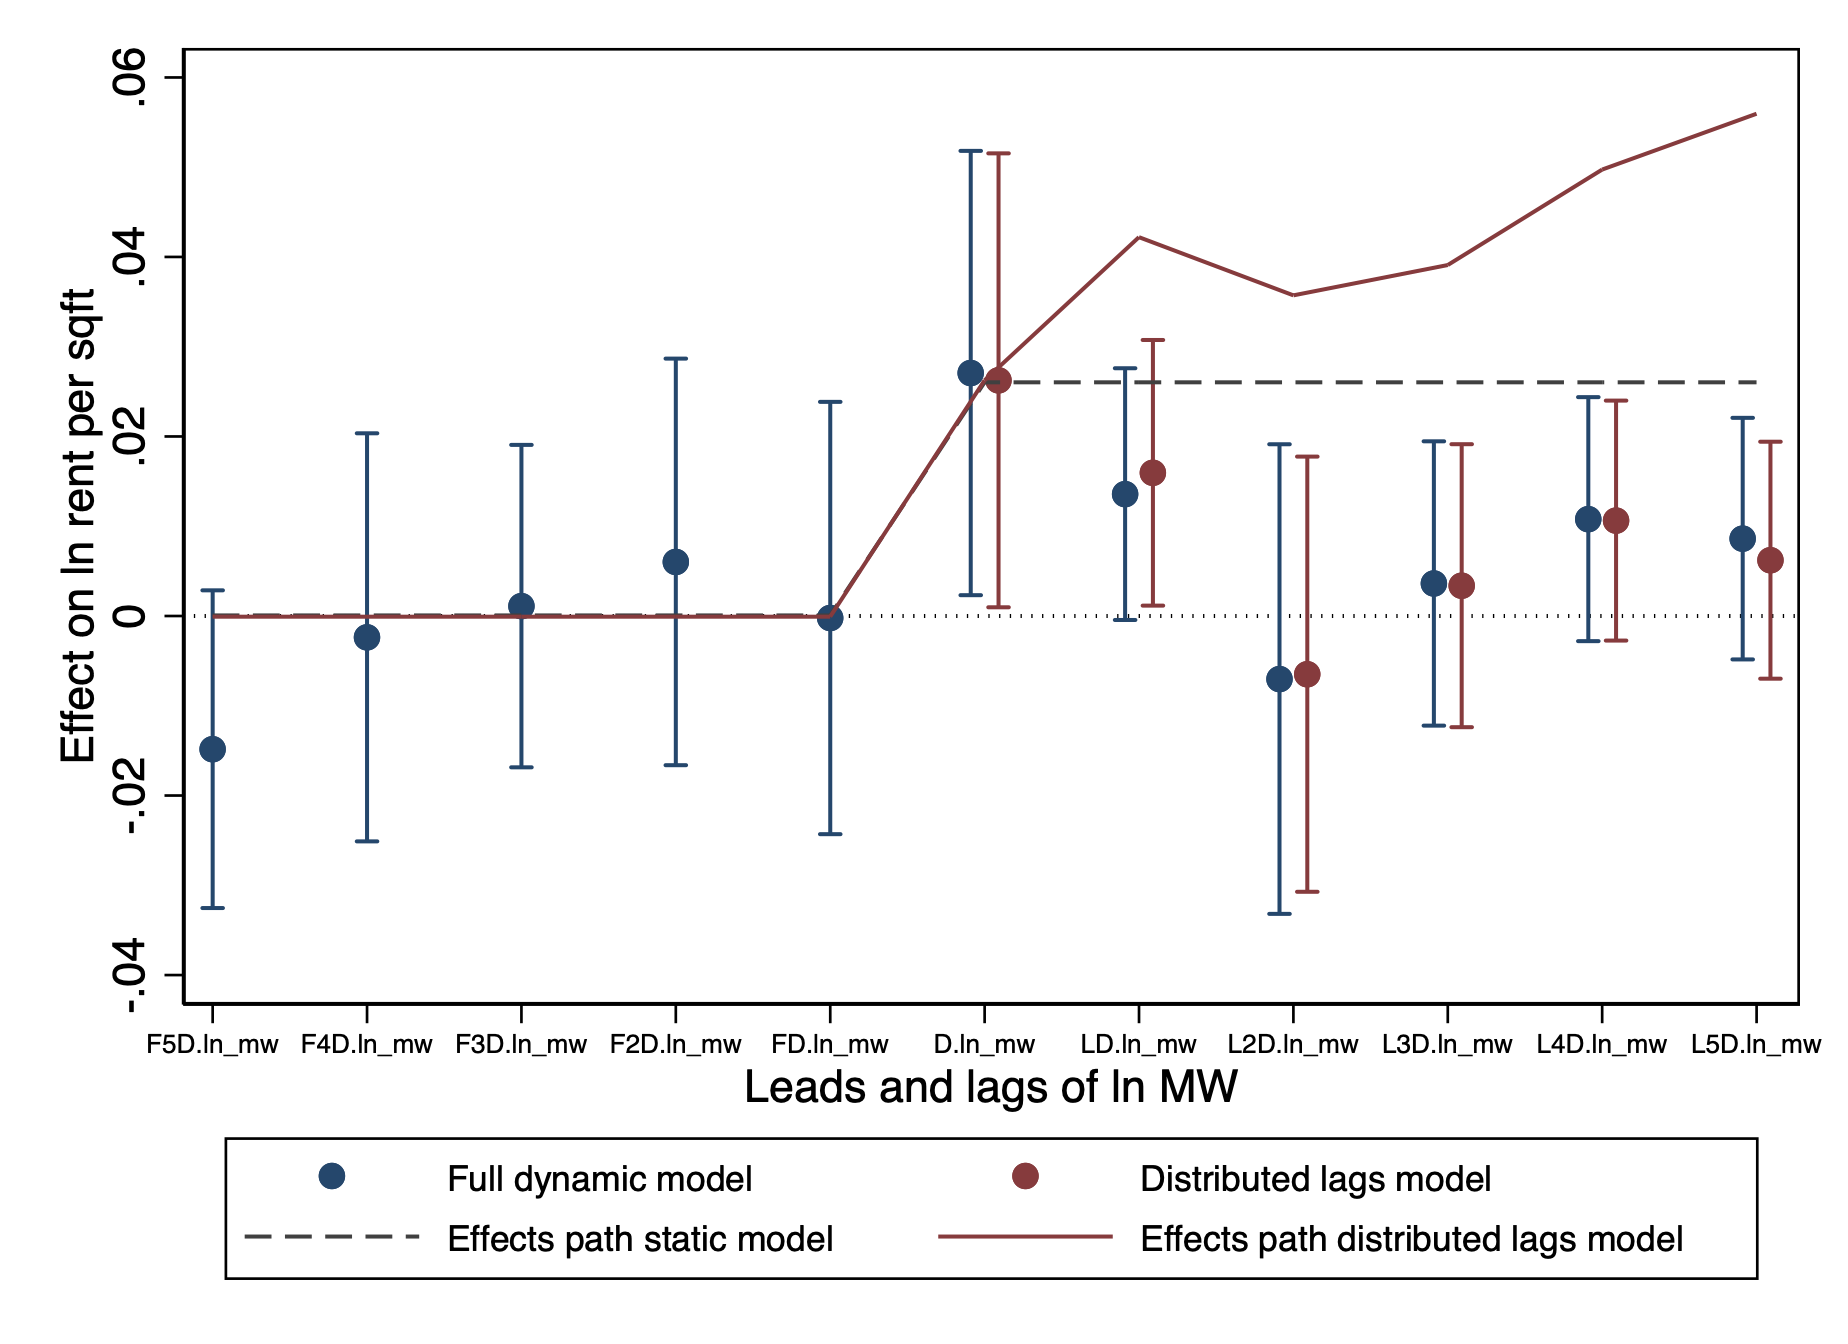
\includegraphics[width = 0.8\textwidth]{../analysis/first_differences/output/fd_models.png}
    \begin{minipage}{0.95\textwidth} \footnotesize
		\vspace{2mm} 
		\textit{Notes}: The plot shows the estimated coefficients for the \textit{dynamic DiD} 
		models estimated through \autoref{eq:leads_lags} and (\ref{eq:lags}) alongside 90 percent 
		confidence intervals. The dashed line additionally reports the point estimate from the 
		\autoref{eq:did}. The solid red line show the point estimates for the cumulative effects 
		estimated through the distributed lags model in \autoref{eq:lags}. Standard errors for both 
		the \textit{static} and the final period of the distributed lag models are reported in 
		\autoref{tab:did_main} and \autoref{tab:dynamic_cumulative} respectively. 
	\end{minipage}
\end{figure}

We summarize and compare the results from the \textit{static} and the \textit{dynamic} DiD models 
in \autoref{fig:fd_models_main}. The dashed line shows the effect path on rents implied by the 
point estimates (the standard error is omitted to avoid cluttering the figure) from the static DiD 
(equation \ref{eq:did}). The blue-dot series plots the estimates from \autoref{eq:leads_lags}, where 
we can appreciate the absence of pre-trends and that the bulk of the effect is concentrated in the 
first two periods. We also report the estimated coefficients from the dynamic model defined in 
\autoref{eq:lags} (red-dot series), showing how the estimates mimic closely those found with the 
leads and lags model. Finally, with the continuous red line we show the cumulative effect of MW 
changes on rents implied by the red dots. As stated before, the effects implied by the dynamic models 
are larger than the ones implied by the static DiD.

To directly account for the presence of zipcode level rent dynamics, we further test our results by 
estimating a \textit{dynamic} DiD model that controls for the lagged value of the changes in rents 
(equation \ref{eq:ab_panel}). We compare that with our baseline estimates in 
\autoref{tab:horse_race_main}: columns 1, 2, and 3 show coefficients from equations \eqref{eq:did}, 
\eqref{eq:leads_lags}, and \eqref{eq:lags} respectively. In columns 4 and 5, we allow for full blown 
dynamics in the dependent variable and we recover the coefficients using instrumental variables 
following the classic \textcite{arellano1991some} approach --using deeper lags of the dependent 
variable to instrument for the lagged dependent variable-- for the cases with and without leads. 
In columns 6 and 7 we show estimates from the model in equation \ref{eq:ab_panel} but instrumenting 
the lagged dependent variable with the sixth MW change lag as in \textcite{meer2016effects}. Our 
effects are robust to all of this stringent tests: the same-month change in rents following a 10 
percent increase in MW is consistently estimated between 0.25 and 0.3 percent. 


\subsection{External Validity and Data Sensitivity}\label{sec:sample_rest}

Our results suggest a noticeable impact of MW policies on the rental housing market. However, as 
explained in \autoref{sec:data}, the number of zipcodes included in the final sample is only a 
small portion of the total U.S., and they come from more urban and richer neighborhoods that likely 
have a dynamic housing market. This limited sample size might hinder the external validity of the 
estimated effect. Additionally, the zipcodes included in the final sample are the ones appearing 
earlier in the Zillow data (i.e. zipcodes whose rent data are available since January 2010), and 
this might result in unobserved differences affecting sample selection.

We test the sensitivity with respect to our sample restrictions in two ways. First, we extend our 
panel by including the full set of zipcodes for which there is available rent data. This, on one 
hand, doubles the sample size (we now use the full $3,316$ zipcode in the Zillow rent data for 
single family, condos and cooperative houses), but, on the other hand, makes the composition of 
zipcodes vary over time by including, as they enter the sample, zipcodes whose time series start 
later than January 2010. Therefore, to fully exploit our data we estimate models using an unbalanced 
panel but controlling for ``cohort $\times$ period" fixed effects. We do this for our main 
specifications in equations \eqref{eq:did}, \eqref{eq:leads_lags}, and \eqref{eq:lags}. In this way, 
we are able to compare treated and untreated zipcodes with the same panel length. In 
\autoref{tab:comparison_unbal_base} we show that that the estimated effects for the different models 
remain widely unchanged. In \autoref{fig:dynamic_dd_comparison}, panel (a) we compare 
\textit{dynamic} DiD estimates obtained using the baseline sample and the unbalanced sample. Using 
the unbalanced panel, our estimates are slightly lower but they are largely identical to the baseline 
results.

Secondly, we assess the representativeness of our estimates by re-weighting zipcodes so as to match 
socio-demographic characteristics of the zipcodes in the top-100 CBSA. We do this by applying the 
entropy balancing procedure developed by \cite{hainmueller2012entropy} on the following zipcode 
level demographics: share of rental houses, share of African-American residents, share of college 
graduates, and median income. We target averages from \autoref{tab:desc_stats}, column 
2.\footnote{The entropy balancing procedure consists of a re-weighting scheme that assigns a scalar 
	weight to every unit such that the re-weighted sample matches moments of a target population. We 
	implement this by leveraging the \texttt{STATA} package \texttt{ebalance} described in 
	\textcite{hainmueller2013ebalance}.} 
We subsequently re-estimate our models with weighted regressions.

The results shown in \autoref{fig:dynamic_dd_comparison}, panel(b) confirm what we found in our 
baseline case, although point estimates are somewhat higher. Note that the simultaneous effect from 
the \textit{dynamic} DiD model presents the only statistically significant post-treatment 
coefficient. The effect in month $t+1$ becomes indeed smaller and not significant, suggesting how 
the baseline model might overestimate the persistence of the true average effect. A comparison with 
the \textit{static} DiD estimate supports this finding: $\hat{\beta}$ from \autoref{eq:did} and 
$\hat{\beta}_{t}$ from \autoref{eq:leads_lags} are almost identical, identifying an elasticity on 
rents of approximately $0.036$ (\autoref{tab:comparison_wgt_base}).

\begin{figure}[htb!]
    \caption{Comparison between dynamic DiD models}
    \label{fig:dynamic_dd_comparison}
    \centering
    \begin{subfigure}[b]{0.8\textwidth}
        \caption{Unbalanced panel}
        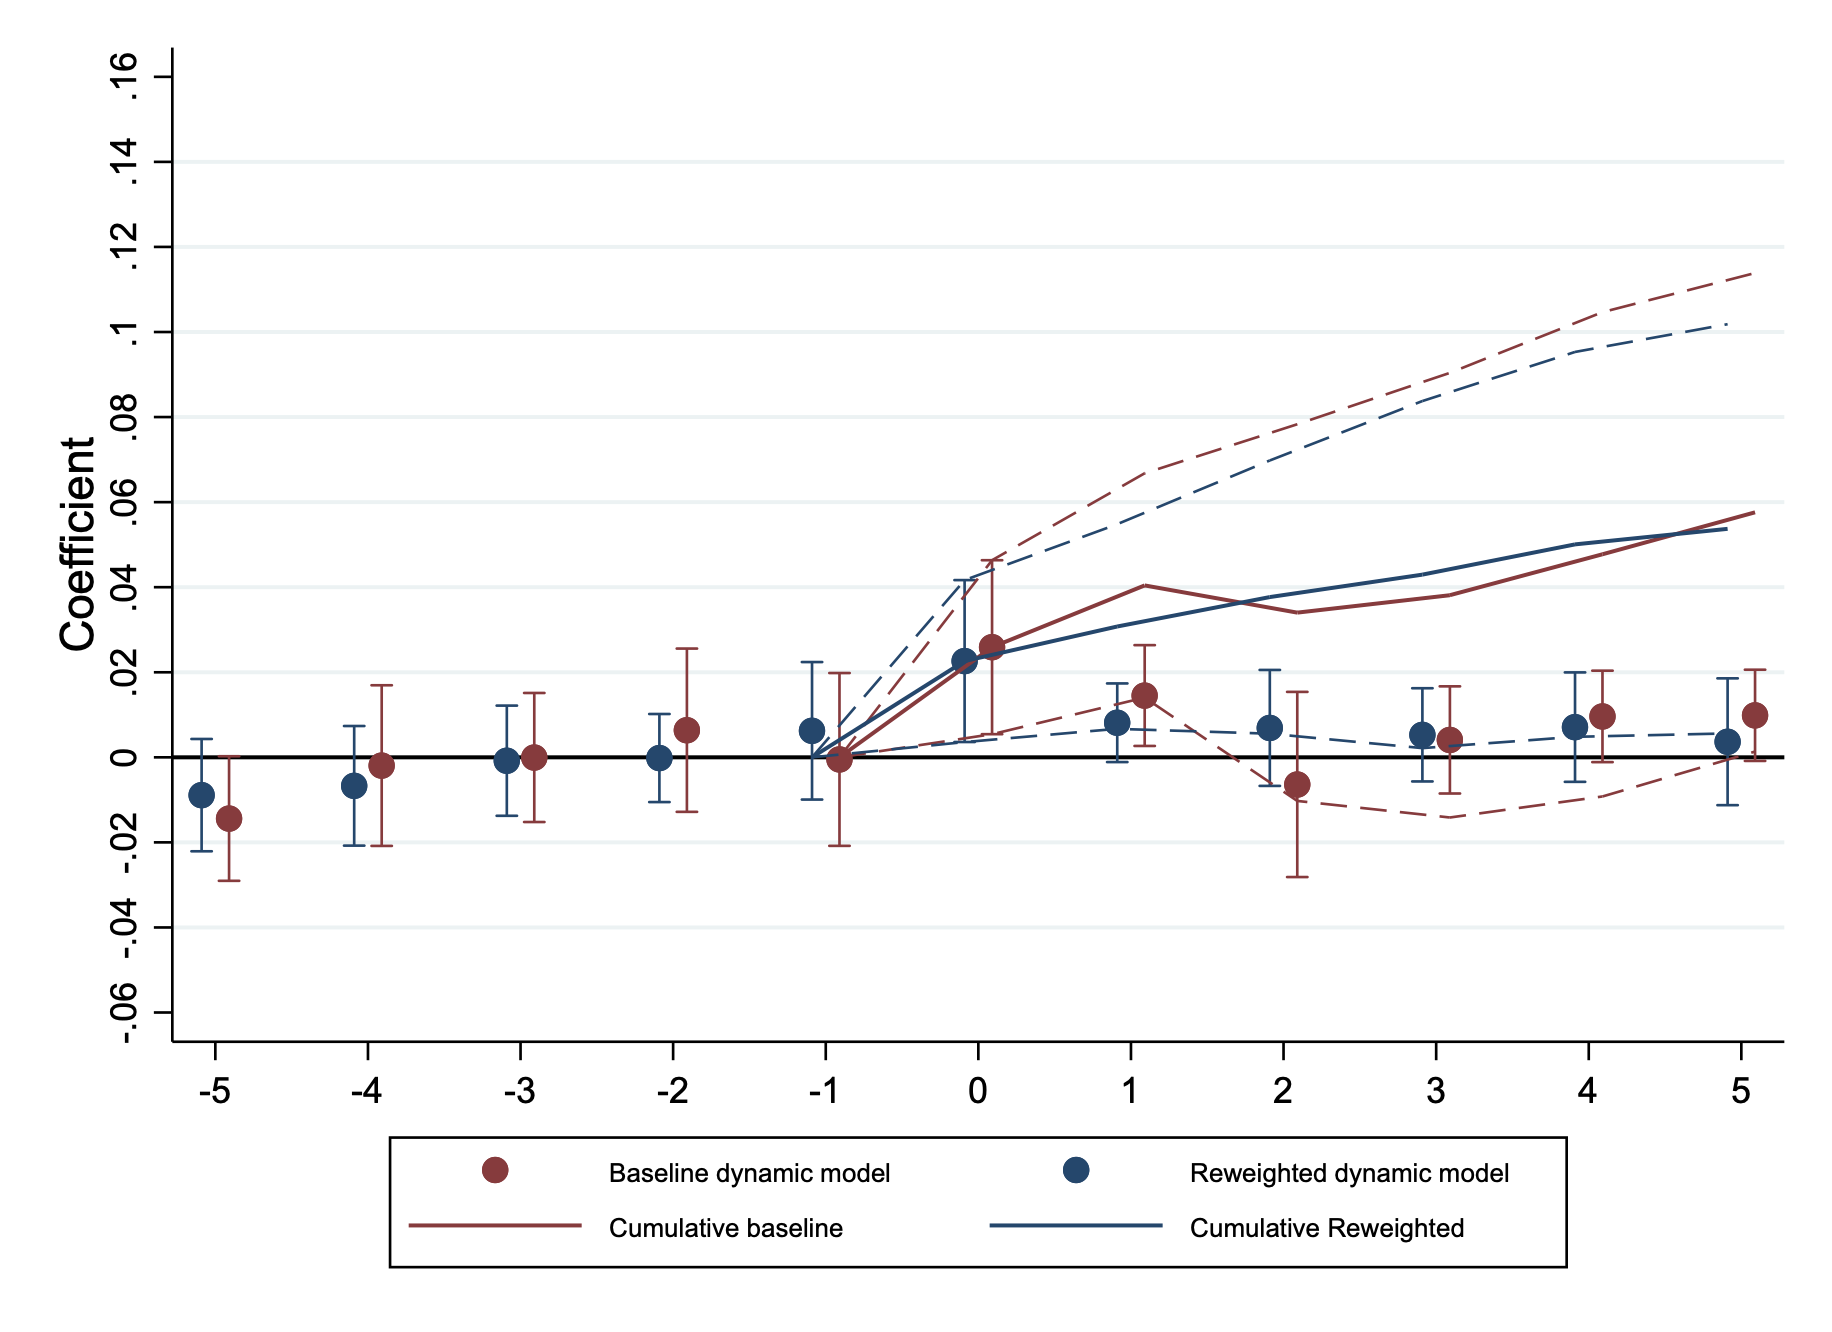
\includegraphics[width = \textwidth]
        {../analysis/first_differences_unbal/output/fd_model_comparison_unbal.png}
    \end{subfigure}
    \begin{subfigure}[b]{0.8\textwidth}
        \caption{Reweighted panel}
        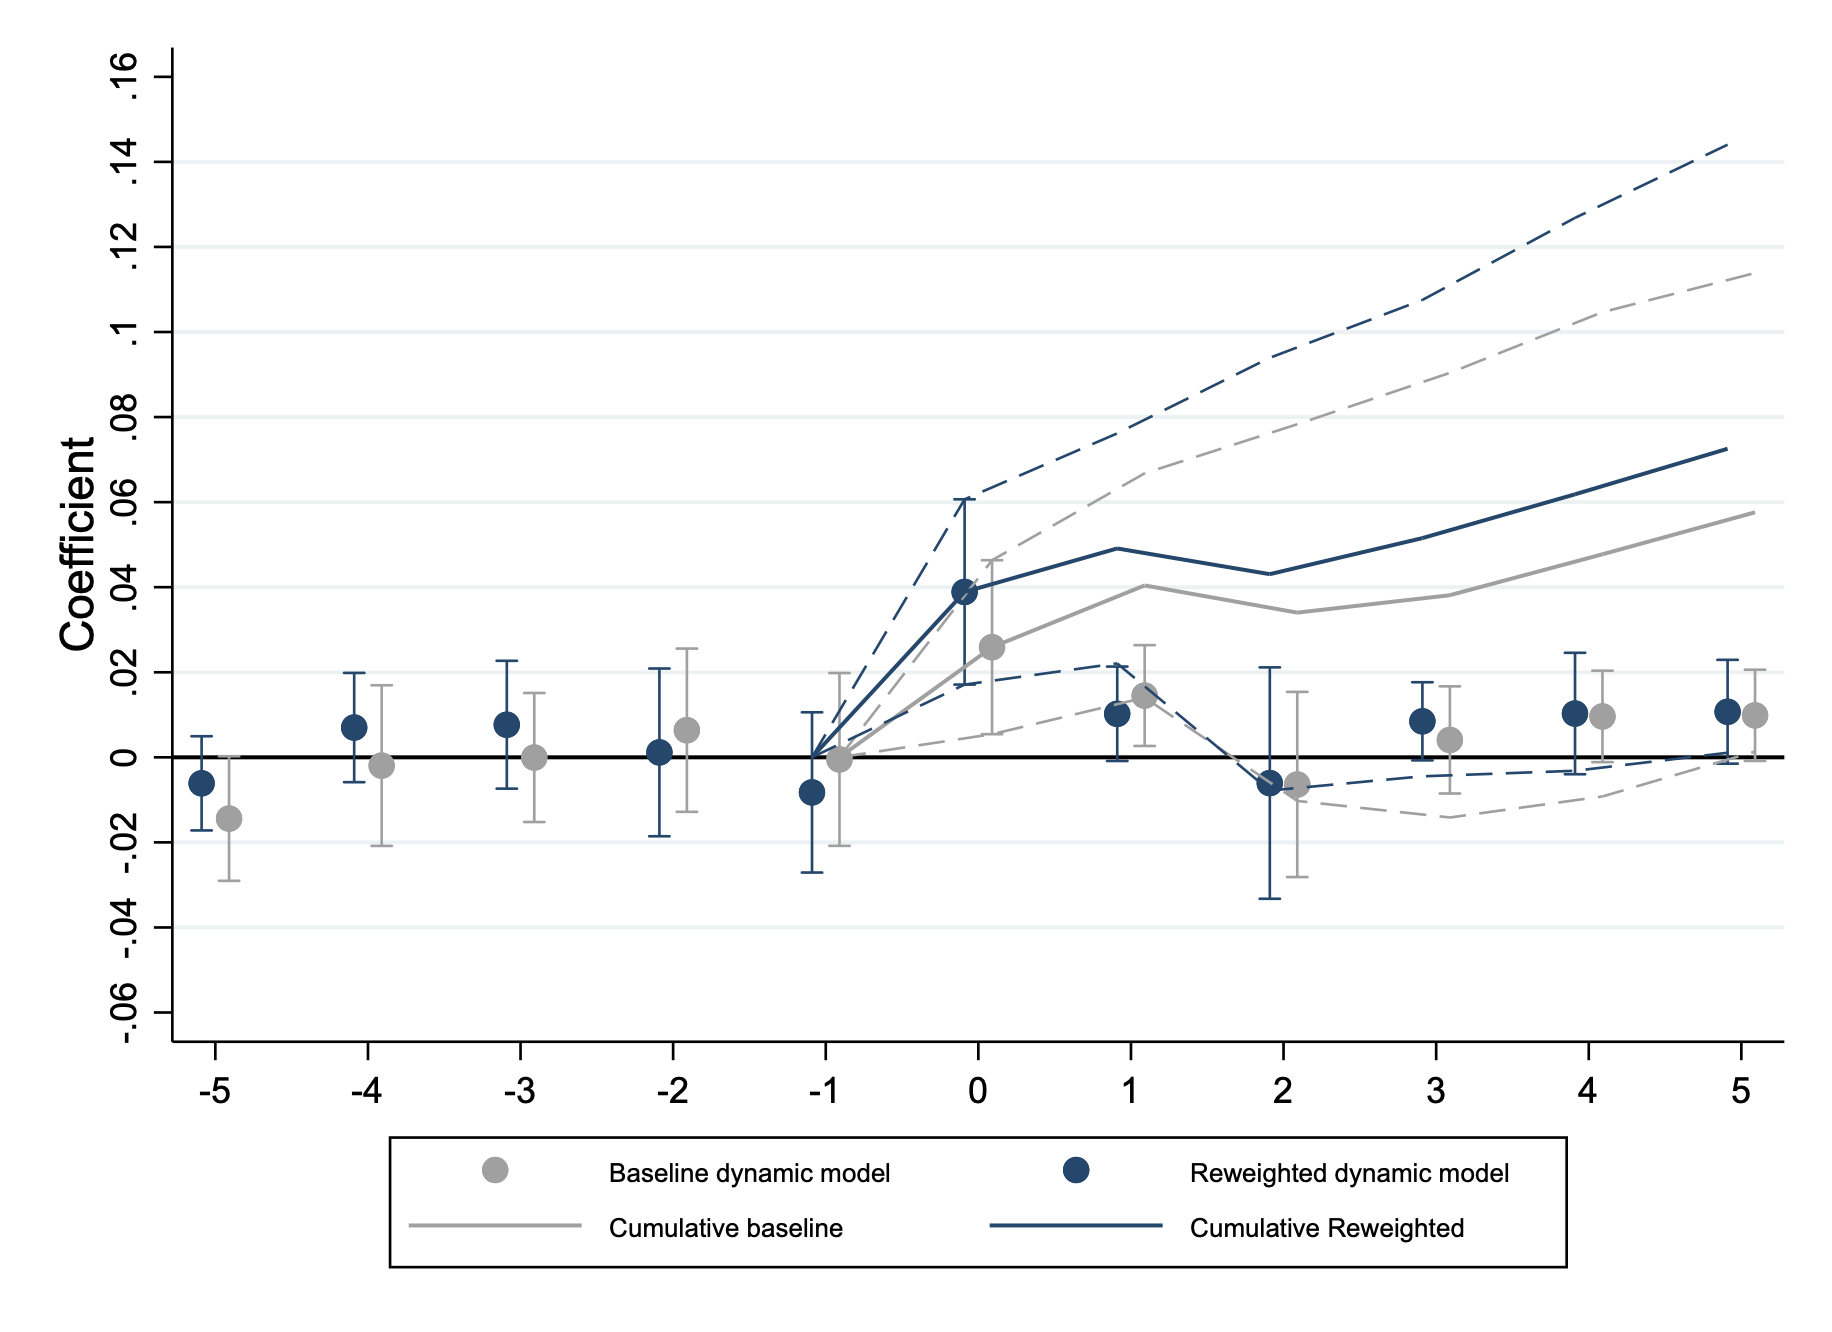
\includegraphics[width = \textwidth]
        {../analysis/first_differences_wgt/output/fd_model_comparison_wgt.png}
    \end{subfigure}
    \begin{minipage}{0.95\textwidth} \footnotesize
		\vspace{2mm} 
		\textit{Notes}: The plot compares results obtained from the baseline panel summarized in 
		\autoref{tab:desc_stats}, column 4 with those obtained from the full unbalanced panel (a), 
		and with the reweighted baseline panel (b). Each subfigure compares estimated coefficients 
		for the \textit{dynamic DiD} models calculated through \autoref{eq:leads_lags}, and point 
		estimates for the cumulative effect of MW on rents estimated through \autoref{eq:lags}.   
	\end{minipage}
\end{figure}


%%%%%%%%%%%%%%%%%%%%%%%%%%%%%%%%%%%%%%%%%%%%%%%%%%%%%%%%%%%%%%%%%%%%%%%%%%%%%%%%%
\subsection{The Role of Unobserved Local Shocks}\label{sec:econ_shocks}

In \autoref{sec:baseline_results} we used \autoref{eq:leads_lags} to establish the absence of 
significant pre-trends in rent dynamics. Another potential threat to the identification of the true 
causal effect might come from unobserved local shocks systematically affecting MW and rent changes. 
In order to account for that, we directly control for proxies of general economic shocks, as well as 
shocks related to the labor and housing markets aggregated at either the county-month or 
county-quarter level, while rents are defined at the zipcode-level. While this prevents us from 
studying the presence of zipcode-level time-varying confounding factors, it substantially strengthens 
the robustness of the estimated impact since the treatment is administered at city, county, or state 
level. In fact, if there are underlying factors affecting MW changes that also affect zipcode-level 
rents, they would likely arise from this larger geographic units.

Controls included in our regressions are the following. First, to account for local economic shocks, 
we use the county-quarter number of establishments by industry obtained from the QCEW (see 
\autoref{sec:data} for more details). We then proxy for local labor market dynamics with two sets 
of controls: county-quarter weekly average wage, and county-month employment by industry. Since we 
are using a first-difference specification, we augment each model with their log difference. Second, 
we proxy for shocks that may stem from the housing market using the county-month number of new 
permits for residential one-unit buildings and the associated permits' valuation. Since these two 
series already report changes between periods, we only control for the log levels.

\begin{table}[h!]
    \caption{Results from Difference-in-Differences model with leads and lags and controls}
    \label{tab:dynamic_leads_lags_econshock}
    \centering
    \resizebox{0.9\textwidth}{!}{
	    \vspace{0pt}
	    {
\def\sym#1{\ifmmode^{#1}\else\(^{#1}\)\fi}
\begin{tabular}{l*{5}{c}}
\hline\hline
          &\multicolumn{1}{c}{(1)}&\multicolumn{1}{c}{(2)}&\multicolumn{1}{c}{(3)}&\multicolumn{1}{c}{(4)}&\multicolumn{1}{c}{(5)}\\
          &\multicolumn{1}{c}{D.ln\_med\_rent\_psqft}&\multicolumn{1}{c}{D.ln\_med\_rent\_psqft}&\multicolumn{1}{c}{D.ln\_med\_rent\_psqft}&\multicolumn{1}{c}{D.ln\_med\_rent\_psqft}&\multicolumn{1}{c}{D.ln\_med\_rent\_psqft}\\
\hline
F5D.ln\_mw &  -0.0157         &  -0.0150\sym{*}  &  -0.0150\sym{*}  &  -0.0146\sym{*}  &  -0.0191\sym{*}  \\
          &(0.00938)         &(0.00832)         &(0.00816)         &(0.00823)         &(0.00983)         \\
[1em]
F4D.ln\_mw & -0.00382         & -0.00125         & -0.00131         & -0.00114         & -0.00776         \\
          & (0.0101)         &(0.00874)         &(0.00875)         &(0.00873)         &(0.00938)         \\
[1em]
F3D.ln\_mw &-0.000214         & -0.00150         & -0.00179         & -0.00133         &  0.00420         \\
          &(0.00831)         &(0.00889)         &(0.00910)         &(0.00885)         &(0.00917)         \\
[1em]
F2D.ln\_mw &  0.00477         &  0.00200         &  0.00219         &  0.00263         &  0.00276         \\
          & (0.0115)         & (0.0115)         & (0.0116)         & (0.0117)         & (0.0133)         \\
[1em]
FD.ln\_mw  & -0.00143         & -0.00398         & -0.00397         & -0.00394         &  -0.0114         \\
          & (0.0142)         & (0.0146)         & (0.0145)         & (0.0145)         & (0.0167)         \\
[1em]
D.ln\_mw   &   0.0260\sym{**} &   0.0265\sym{**} &   0.0269\sym{**} &   0.0258\sym{**} &   0.0267\sym{*}  \\
          & (0.0110)         & (0.0113)         & (0.0108)         & (0.0105)         & (0.0140)         \\
[1em]
LD.ln\_mw  &   0.0118         &   0.0108         &   0.0112         &   0.0115         &   0.0169\sym{**} \\
          &(0.00805)         &(0.00834)         &(0.00859)         &(0.00878)         &(0.00752)         \\
[1em]
L2D.ln\_mw & -0.00884         & -0.00554         & -0.00561         & -0.00548         & -0.00101         \\
          & (0.0124)         & (0.0126)         & (0.0127)         & (0.0127)         & (0.0143)         \\
[1em]
L3D.ln\_mw &  0.00191         &  0.00324         &  0.00326         &  0.00453         &  0.00845         \\
          &(0.00812)         &(0.00821)         &(0.00829)         &(0.00795)         &(0.00837)         \\
[1em]
L4D.ln\_mw &  0.00918         &   0.0105         &   0.0108         &  0.00968         &   0.0105         \\
          &(0.00724)         &(0.00686)         &(0.00680)         &(0.00683)         &(0.00675)         \\
[1em]
L5D.ln\_mw &  0.00736         &  0.00743         &  0.00749         &  0.00748         &  0.00702         \\
          &(0.00717)         &(0.00785)         &(0.00782)         &(0.00775)         &(0.00834)         \\
\hline
P-value no pretrends&    0.602         &    0.632         &    0.609         &    0.633         &    0.514         \\
Industry-level monthly employment&       No         &      Yes         &      Yes         &      Yes         &      Yes         \\
Industry-level quarterly establishment count&       No         &       No         &      Yes         &      Yes         &      Yes         \\
Industry-level quarterly weekly wage&       No         &       No         &       No         &      Yes         &      Yes         \\
New housing permits and value&       No         &       No         &       No         &       No         &      Yes         \\
R-squared &    0.027         &    0.028         &    0.028         &    0.028         &    0.031         \\
Observations&   106446         &   101448         &   101448         &   101448         &    82716         \\
\hline\hline
\end{tabular}
}
}
    \begin{minipage}{0.95\textwidth} \footnotesize
		\vspace{3mm} 
		\textit{Notes}: The table reports coefficients from \autoref{eq:leads_lags} estimated on the 
		balanced panel of zipcode-months that contains SFCC rental price. All specifications include 
		zipcode linear trends. Column (1) replicates our baseline results from 
		\autoref{tab:dynamic_lags_leads_main}, column 2. Columns 2 to 5 progressively add sets of 
		time-varying covariates that control for local shocks. Columns 2 to 4 add controls for the 
		following industries: goods-producing; natural resources and mining; construction; 
		manufacturing; service-providing; trade, transportation and utilities; information; 
		financial activities; professional and business services; education and health services; 
		leisure and hospitality. They additionally control for federal, state, and local government. 
		Standard errors clustered at the state level. *** $p < 0.01$, ** $p < 0.05$, * $p < 0.1$.
	\end{minipage}
\end{table}

In \autoref{tab:dynamic_leads_lags_econshock} we report the estimated coefficients for 
\autoref{eq:leads_lags}, progressively increasing the set of controls included in the regression. 
Column 1 replicates our baseline results (\autoref{tab:dynamic_lags_leads_main}, column 2); columns 
2 to 5 show estimated coefficients when adding all the aforementioned covariates. The estimated 
impact of MW changes remains substantially unchanged regardless of the set of controls used: we 
consistently observe that a 10 percent increase in MW causes a simultaneous increase in rents of 
approximately 0.26 percent. Only in column 5 we cannot reject the null hypothesis that 
$\hat{\beta}_{t} = 0$, as the points estimate slightly decreases while the smaller sample size leads 
to higher standard errors, but the coefficient on $t+1$ is also larger and significant. A quick 
comparison with leads and lags however clearly indicates the unchanged nature of our results. The 
inclusion of this relevant controls reveals the presence of a very mild pre-trend, however, we note 
that the joint F-test on all leads still fails to reject that they are all zero.   


%%%%%%%%%%%%%%%%%%%%%%%%%%%%%%%%%%%%%%%%%%%%%%%%%%%%%%%%%%%%%%%%%%%%%%%%%%%%%%%%%
\subsection{Benchmarking}\label{sec:benchmark}
TO ADD


%%%%%%%%%%%%%%%%%%%%%%%%%%%%%%%%%%%%%%%%%%%%%%%%%%%%%%%%%%%%%%%%%%%%%%%%%%%%%%%%%
\subsection{The Heterogeneity of MW Impacts on Rents}\label{sec:heter}

Our baseline results in \autoref{sec:baseline_results} have documented the presence of a causal 
impact of MW on rents, and the effect appears robust to multiple checks introduced in Sections 
\ref{sec:sample_rest} and \ref{sec:econ_shocks}. We now investigate the heterogeneity of such effect 
by characterizing zipcodes based on socio-demographic characteristics. The goal of this exercise is 
twofold: first, MW is a place-based policy targeted to a specific sub-population that does not 
necessarily live and work in the same zipcode. The presence of a significant effect in treated 
zipcodes does not reveal whether MW workers are actually bearing the burden of this increase, or if 
instead rents increase in those zipcodes where MW jobs are concentrated. We therefore try to answer 
the following question: do rents increase more where MW workers live, or where they work? second, 
independently from the incidence on MW workers, who are the winners and losers when rents increase 
due to new MW provisions? we look at zipcode characteristics to identify which sub-population ends 
up paying more in rents.

To answer the first question it requires to localize MW workers job and residence locations at the 
zipcode level. While direct data on this feature of zipcodes is not available, we build proxies 
based on the LODES data. Specifically, we use the 2017 files to compute the share (out of state 
totals) of low-income workers under 30 years old that either live or work in any given zipcodes (MW 
workplace and residence distribution henceforth).\footnote{See \autoref{sec:data} for more details 
	on the construction of such variables.} 
Since the majority of the MW changes in our data are at the state-level, we calculate shares over 
state totals so that we are able to study the impact of this type of policy on the relevant 
distribution of low-income, young workers. While these proxies by definition include more than MW 
workers, \cite{dube2016minimum} show how MW changes actually affect a larger part of the income 
distribution than just workers below MW thresholds (a statistically significant impact on wages is 
reported up to $\$4$ above the new MW thresholds). We then bin each state distribution into quartiles 
and use \autoref{eq:diff_main_hetero} to estimate the differential effect for each group.

\begin{figure}[h!]
    \caption{Static DiD model: MW impact by workers job and residence location}
    \label{fig:static_dd_workers_home_work}
    \centering
    \begin{subfigure}[b]{0.6\textwidth}
        \caption{Workplace location}                  %%% CHANGE INPUT FOLDER
        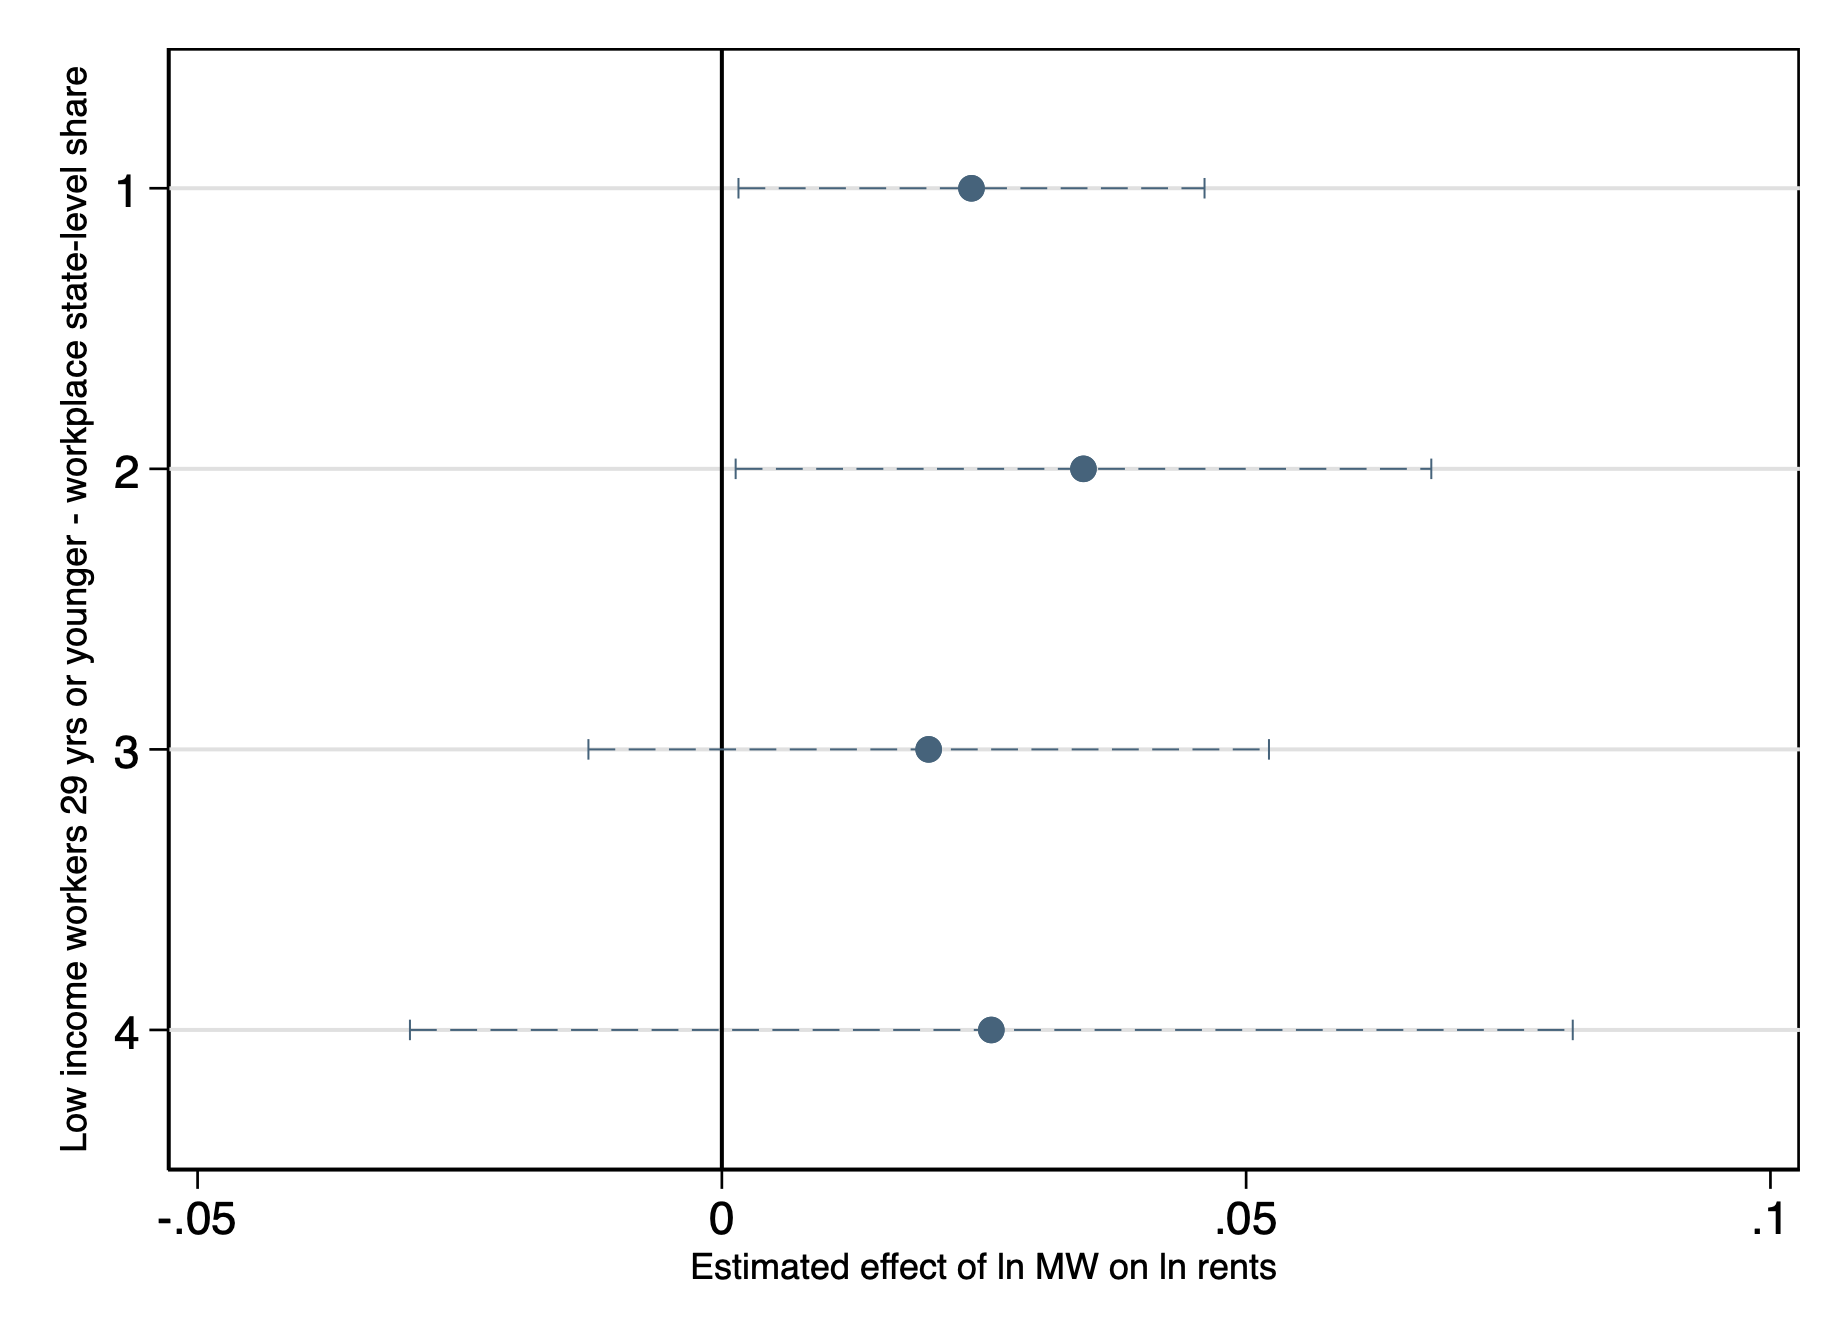
\includegraphics[width = \textwidth]{input/fd_static_heter_walall_29y_lowinc_ssh.png}
    \end{subfigure}
    \begin{subfigure}[b]{0.6\textwidth}
        \caption{Residence location}
        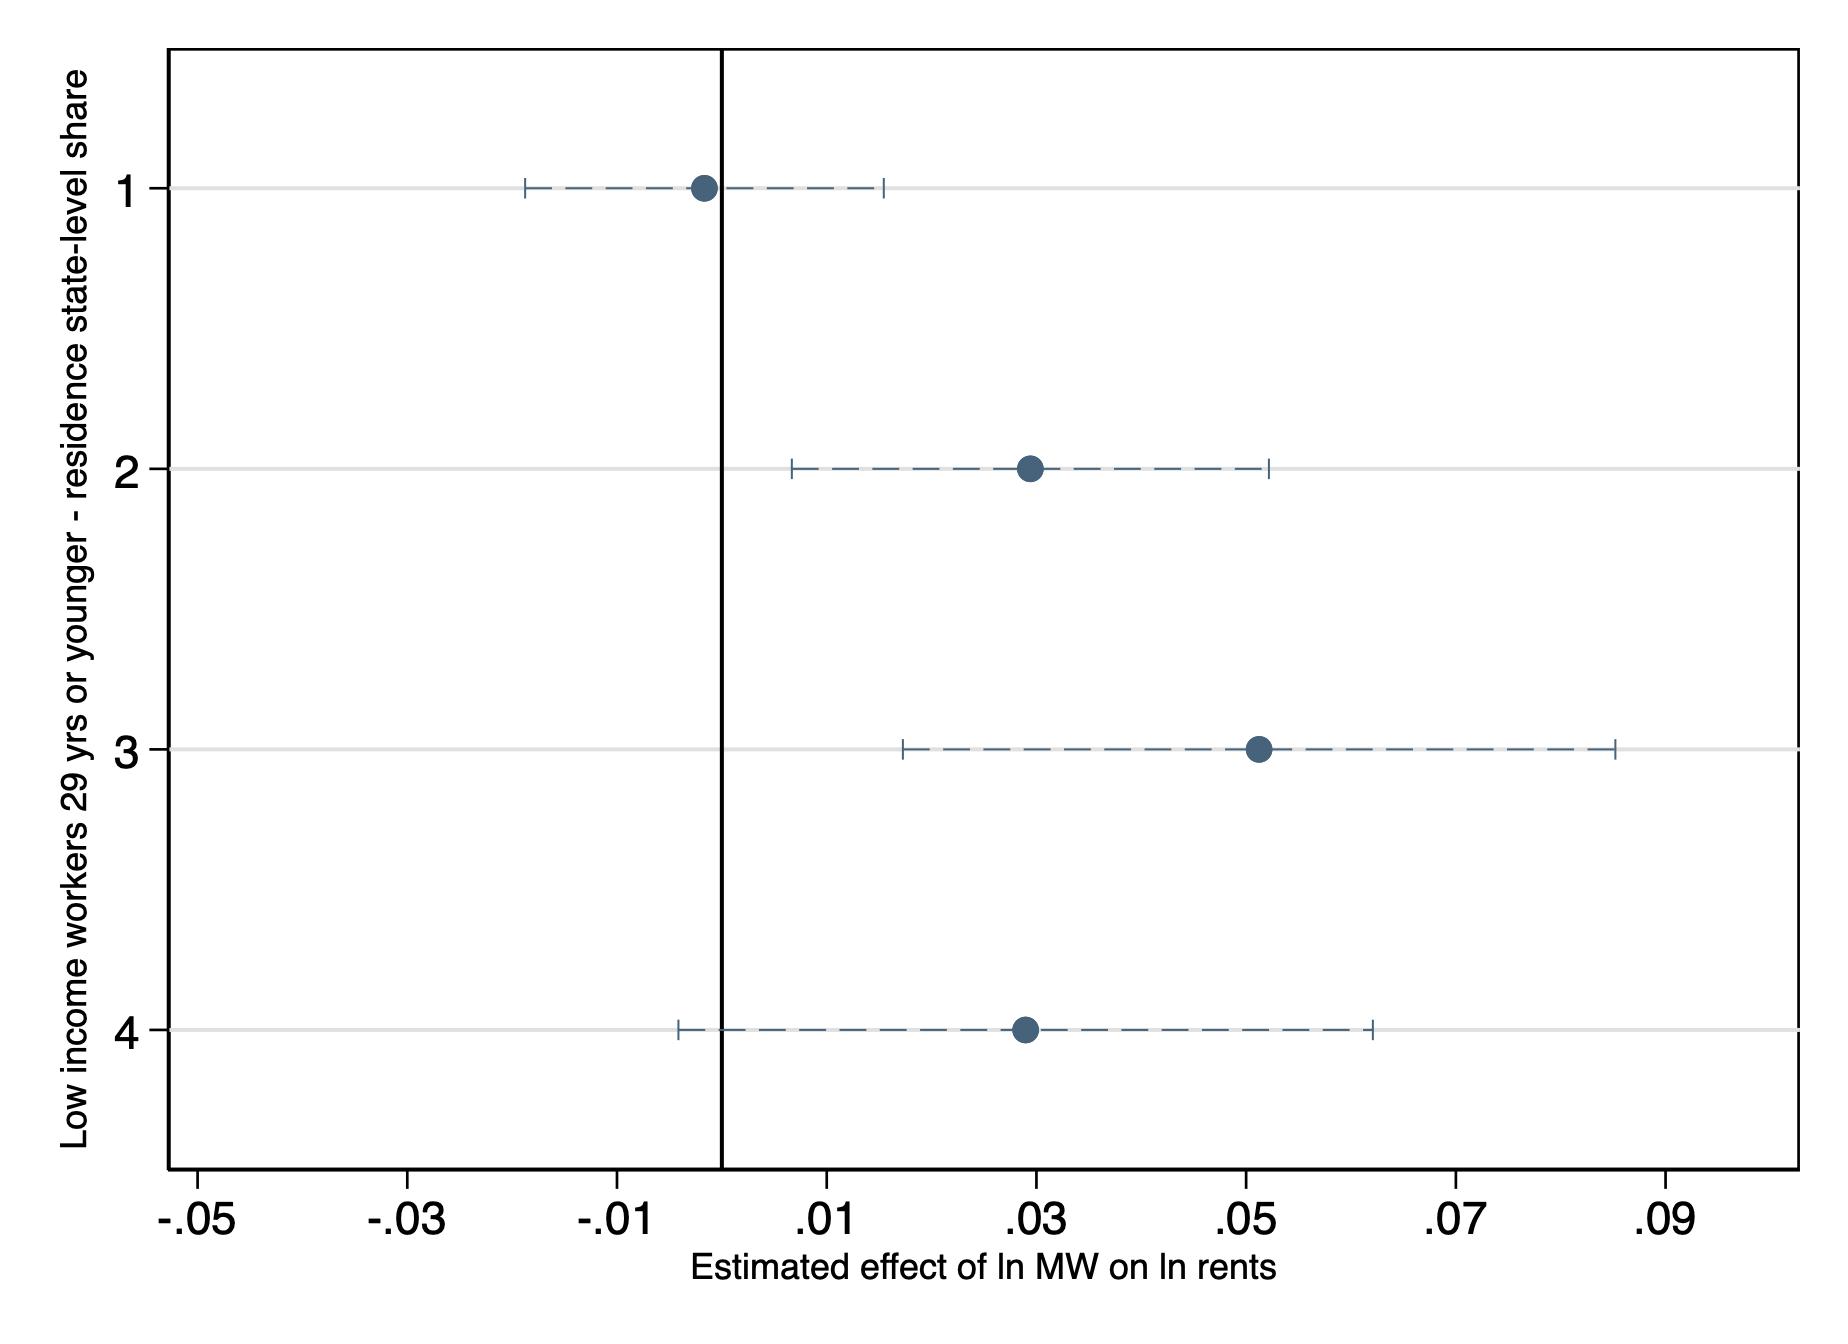
\includegraphics[width = \textwidth]{input/fd_static_heter_halall_29y_lowinc_ssh.png}
    \end{subfigure}
    \begin{minipage}{0.95\textwidth} \footnotesize
		\vspace{2mm} 
		\textit{Notes}: The Figure shows the estimated coefficients $\beta_{q}$, $q \in \{1, 2, 3,
		4\}$ from \autoref{eq:diff_main_hetero} when differentiating zipcodes with respect to the 
		share of MW workers that either work (a) or live (b) in each zipcode. Shares are taken over 
		state totals. MW workers is used as a loose label for workers below 30 years old earning 
		less than $\$1250$ month identified using the 2017 LODES datasets (see \autoref{sec:data} 
		for more information). 90 percent confidence intervals reported.
	\end{minipage}
\end{figure}

In \autoref{fig:static_dd_workers_home_work} we plot the estimated coefficients for the interaction 
between changes in (log) MW and each quartile of the two distributions. Panel (a) presents results 
for MW workplace location. The point estimates are very similar, suggesting that the effect on rents 
is orthogonal to the geographic distribution of MW workplace. The coefficients for the first 2 
quartiles are significant at the $10$ percent level, but standard errors for the $3^{rd}$ and 
$4^{th}$ quartiles become very large partly due to a heavily right-skewed distribution of the 
underlying variable. In panel (b) we re-estimate \autoref{eq:diff_main_hetero} using the MW residence 
distribution. Here we do observe a different pattern: the point estimate in the lowest quartile is 
precisely zero, but this increases and becomes statistically significant both in the $2^{nd}$ and 
$3^{rd}$ quartile. Even more, the effect appears larger: a 10 percent increase in MW leads to a 0.5 
percent increase in rents. The estimated effect for zipcodes with the highest share of young, 
low-income workers decreases to 0.3 percent and becomes not significant, but we notice how also the 
underlying MW residence distribution is heavily right-skewed, and this higher variance partially 
justify the lower precision in our estimates. Overall, this exercise shows how MW workers indeed seem 
to bear most of the impact with relatively higher rents in their place of residence.

The LODES-based proxies for MW workers are approximate by definition. We then turn to investigate 
how the impact of MW changes on rents differs across the distribution for different census-based 
zipcode demographics. The Bureau of Labor Statistics reports how MW workers tend to be young and 
less educated.\footnote{See, for example, BLS Report 1085, \textit{Characteristics of Minimum Wage 
		Workers 2019} at \url{https://www.bls.gov/opub/reports/minimum-wage/2019/home.htm}} 
The study of heterogeneous effects by demographics can therefore help both in confirming what the
LODES-based measures indicate, and in uncovering additional patterns of the effects under study.

\autoref{tab:fd_model_het} shows the estimated coefficients for the interaction between changes in 
(log) MW and quartiles of the distribution for several demographics. In column 1 we show how the 
effect disproportionately impact zipcodes in the lowest quartile of the median income distribution: 
the estimated elasticity of rent to MW is 0.039 (s.e. 0.022). The effect on the other quartiles 
becomes not significant and it shows a non-monotone behavior in the $2^{nd}$ and $3^{rd}$ quartiles. 
When looking at the richest neighborhoods however, we have a markedly smaller and imprecise estimate. 
In column 2 we focus on the zipcode-level unemployment  rate. Not surprisingly, we find that the 
strongest effect is localized in the $4^{th}$ quartile of the distribution, 0.045 (s.e. 0.017). 
Estimates lose significance in the remaining part of the distribution: similarly to column 1, we 
find not-significant not-monotone estimates in the middle quartiles, while the effect is a clear 
zero in the bottom quarter. In column 3 we look at the share of college graduates, and the estimates 
confirm that indeed lower educated neighborhoods bear the bulk of the rent increase: there is a 
clear divide between above median zipcodes showing zero and not significant effects, and below 
median ones where a 10 percent increase in MW leads to a 0.47 and a 0.37 percent rent increase for 
the $2^{nd}$ and $1^{st}$ quartiles, respectively. Lastly, in column 4 we show the impact across 
the distribution over share of African-American residents. Similarly to column 3, we do find a 
stark contrast between above and below median zipcodes. The effect of MW changes on rents 
monotonically increases starting from a not significant effect of 0.017 in the $1^{st}$ quarter to 
a statistically significant 0.042 in the $4^{th}$ one.

\begin{table}[h!]
    \caption{Heterogeneity Results - static DiD model}
    \label{tab:fd_model_het}
    \centering
    \resizebox{0.9\textwidth}{!}{             %%% CHANGE INPUT FOLDER
	    \vspace{0pt}    
	    {
\def\sym#1{\ifmmode^{#1}\else\(^{#1}\)\fi}
\begin{tabular}{l*{6}{c}}
\hline\hline
          &\multicolumn{1}{c}{(1)}&\multicolumn{1}{c}{(2)}&\multicolumn{1}{c}{(3)}&\multicolumn{1}{c}{(4)}&\multicolumn{1}{c}{(5)}&\multicolumn{1}{c}{(6)}\\
          &\multicolumn{1}{c}{\shortstack{Median \\ income}}&\multicolumn{1}{c}{\shortstack{College \\ grad. (\%)}}&\multicolumn{1}{c}{\shortstack{15-24 years \\ old (\%)}}&\multicolumn{1}{c}{\shortstack{African- \\ am. (\%)}}&\multicolumn{1}{c}{\shortstack{Young \\ low-inc. worker,\\ workplace}}&\multicolumn{1}{c}{\shortstack{Young \\ low-inc. worker,\\ residence}}\\
\hline
First quartile&   0.0373         &   0.0356\sym{*}  &   0.0196         &   0.0175         &   0.0214         & -0.00317         \\
          & (0.0223)         & (0.0197)         & (0.0139)         & (0.0159)         & (0.0131)         &(0.00981)         \\
[1em]
Second quartile&   0.0193         &   0.0448\sym{**} &   0.0187         &   0.0217         &   0.0340\sym{*}  &   0.0304\sym{**} \\
          & (0.0146)         & (0.0217)         & (0.0156)         & (0.0157)         & (0.0194)         & (0.0128)         \\
[1em]
Third quartile&   0.0300         &   0.0255         &   0.0212         &   0.0209         &   0.0196         &   0.0498\sym{**} \\
          & (0.0245)         & (0.0208)         & (0.0149)         & (0.0132)         & (0.0187)         & (0.0201)         \\
[1em]
Fourth quartile&   0.0129         &-0.000230         &   0.0414\sym{***}&   0.0404\sym{**} &   0.0249         &   0.0268         \\
          & (0.0126)         & (0.0114)         & (0.0144)         & (0.0162)         & (0.0330)         & (0.0197)         \\
\hline
P-value equality&    0.813         &    0.176         &    0.230         &    0.487         &    0.768         &    0.005         \\
Observations&  107,781         &  107,781         &  107,781         &  107,781         &  107,568         &  107,707         \\
\hline\hline
\end{tabular}
}

    }
    \begin{minipage}{0.95\textwidth} \footnotesize
		\vspace{3mm}
		\textit{Notes}: The table reports estimates for $\beta_{q}$, $q=\{1, 2, 3, 4\}$ from 
		\autoref{eq:diff_main_hetero} when differentiating zipcodes based on several 
		socio-demographics from the 2010 Census and the 5-year 2008-2012 ACS. Standard errors 
		clustered at the state level. *** $p < 0.01$, ** $p < 0.05$, * $p < 0.1$.  
	\end{minipage}
\end{table}


\section{Discussion}\label{sec:discussion}
	%%%%%%%%%%%%%%%%%%%%%%%%%%%%%%%%%%%%%%%%%%%%%%%%%%%%%%%%%%%%%%%%%%%%%%%%%%%%%%%%%
%%%%%                             DISCUSSION                                 %%%%
%%%%%%%%%%%%%%%%%%%%%%%%%%%%%%%%%%%%%%%%%%%%%%%%%%%%%%%%%%%%%%%%%%%%%%%%%%%%%%%%%

In this discussion we discuss the implications of our results.

%%%%%%%%%%%%%%%%%%%%%%%%%%%%%%%%%%%%%%%%%%%%%%%%%%%%%%%%%%%%%%%%%%%%%%%%%%%%%%%%%
\subsection{The magnitude of the estimates}\label{sec:benchmark}

In this subsection we use the model introduced in \autoref{sec:model} combined with some auxiliary 
assumptions to assess whether the magnitude of our estimates is plausible.

Assume that functions that characterize supply and demand of rental units are constant elasticity, 
so that $\underline{\gamma}$ and $\underline{\beta}$ are the elasticity of MW households demand to 
rents and income, $\overline{\gamma}$ and $\overline{\beta}$ are analogous parameters for non-MW 
households, and $k$ is the elasticity of housing supply to rents.\footnote{More precisely, we 
	assume that $\underline{H}(r, \underline{w}) = A e^{\underline{\gamma} \ln r + \underline{\beta} 
		\ln\underline{w}}$, $\overline{H}(r, w) = B e^{\overline{\gamma} \ln r + \overline{\beta} \ln 
		w}$, and $H(r) = C e^{k \ln r}$. $A, B, C > 0$ are constants.}. 
As a result, it can be shown that \autoref{eq:model-elasticity} takes the form

\begin{equation}\label{eq:benchmarking-elasticity}
\rho = \frac{\underline{\beta} \ \underline{s}}
{k - \underline{\gamma} \ \underline{s} 
	- \overline{\gamma} \overline{s}}
\end{equation}
where $\underline{s} = \frac{\underline{H}}{H}$ is share of housing occupied by MW households 
and $\overline{s} = \frac{\overline{H}}{H}$ is the share of housing occupied by non-MW households. 
Note that $\overline{s} = 1 - \underline{s}$.

The above expression is intuitive, in the sense that factors which increase housing demand make 
the elasticity higher, whereas factors that increase supply lower it. For instance, a higher 
$\underline{\beta}$ --elasticity of housing demand to income-- implies a higher $\rho$, whereas 
a higher $k$ --elasticity of housing demand to rents-- implies a lower $\rho$.

Suppose that the share of MW is $\underline{s} = 0.3$, so that $\overline{s}=0.7$. Assume that 
demand elasticities and $(\underline{\gamma}, \overline{\gamma}, \underline{\beta}) = (- 0.7, 
- 0.5, 0.1)$, implying that MW households are more sensible to increases in rents, and that 
demand for housing is price-inelastic and a normal good. Finally, let $k = 0.1$, similar to 
estimate of \textcite[][Table 5]{Diamond2016}. Substituting these values in 
\eqref{eq:benchmarking-elasticity} results in an elasticity of 0.45. This value turns out to be 
very close to the cumulative sum of our $t$ and $t-1$ coefficients.


%%%%%%%%%%%%%%%%%%%%%%%%%%%%%%%%%%%%%%%%%%%%%%%%%%%%%%%%%%%%%%%%%%%%%%%%%%%%%%%%%
\subsection{Policy implications}\label{sec:policy}



\section{Conclusions}\label{sec:conclusion}
    %%%%%%%%%%%%%%%%%%%%%%%%%%%%%%%%%%%%%%%%%%%%%%%%%%%%%%%%%%%%%%%%%%%%%%%%%%%%%%%%%
%%%%%                             CONCLUSION                                 %%%%
%%%%%%%%%%%%%%%%%%%%%%%%%%%%%%%%%%%%%%%%%%%%%%%%%%%%%%%%%%%%%%%%%%%%%%%%%%%%%%%%%

In this paper, we ask whether minimum wage changes affect housing rental prices. To answer this 
question we use rental listings from Zillow and MW changes collected from 
\textcite{vaghul2016historical}, \textcite{cengiz2019effect} and our ourselves, to construct a panel 
at the zipcode-month level. We exploit state, county, and city-level changes in the MW to identify 
the causal impact of increasing the MW. To do that, we leverage on a panel difference-in-differences approach that exploits the staggered implementation and the intensity of hundreds of MW increases 
across thousands of zipcodes. Our results indicate that minimum wage increases have a small but 
significant positive impact on rents that is robust to many alternative explanations. Across most 
specifications, a $10\%$ percent increase in MW causes on average an increase of $0.03 \%$ percent of 
the rental prices. The effect is largely concentrated in the first two months of the MW change. We go 
beyond the average MW effect and we look at the heterogeneity of effects across zipcodes. We show 
that rents disproportionately increase in zipcodes where: (i) it is more likely to find MW workers as 
residents, (ii) there is higher unemployment rate, and (iii) a larger share of African-American 
residents. Our results highlights that place-based policies aimed at the labor market can also have 
significant impacts on other related markets. In particular, MW provisions are usually thought as a 
way to guarantee economic means to low income workers but they may also be benefiting landlords in 
ways that are unintended. In this sense, studying how place-based policies affect the housing market 
becomes an important step to better understand income inequality across U.S. neighborhoods.



 

%%%%%%%%%%%%%%%%%%%%%%%%%%%%%%%%%%%%%%%%%%%%%%%%%%%%%%%%%%%%%%%%%%%%%%%%%%%%%%%%%%
%%%%                                 TAIL                                     %%%%
%%%%%%%%%%%%%%%%%%%%%%%%%%%%%%%%%%%%%%%%%%%%%%%%%%%%%%%%%%%%%%%%%%%%%%%%%%%%%%%%%%

\clearpage
\printbibliography


\clearpage

\section*{\centering{Online Appendix}}
\vspace{5mm}

\appendix

\renewcommand\thetable{\thesection.\arabic{table}}    
\renewcommand\thefigure{\thesection.\arabic{figure}} 
\setcounter{table}{0}
\setcounter{figure}{0}

\section{Appendix Tables}
	%%%%%%%%%%%%%%%%%%%%%%%%%%%%%%%%%%%%%%%%%%%%%%%%%%%%%%%%%%%%%%%%%%%%%%%%%%%%%%%%%
%%%%%                           APPENDIX TABLES                              %%%%
%%%%%%%%%%%%%%%%%%%%%%%%%%%%%%%%%%%%%%%%%%%%%%%%%%%%%%%%%%%%%%%%%%%%%%%%%%%%%%%%%

\begin{table}[h!]
	\caption{Dynamic DiD: cumulative effect over 6 months}
	\label{tab:dynamic_cumulative}
	\centering
	\resizebox{0.7\textwidth}{!}{
		\vspace{0pt}    
		{
\def\sym#1{\ifmmode^{#1}\else\(^{#1}\)\fi}
\begin{tabular}{l*{3}{c}}
\hline\hline
          &\multicolumn{1}{c}{(1)}&\multicolumn{1}{c}{(2)}&\multicolumn{1}{c}{(3)}\\
          &\multicolumn{1}{c}{D.ln\_med\_rent\_psqft\_sfcc}&\multicolumn{1}{c}{D.ln\_med\_rent\_psqft\_sfcc}&\multicolumn{1}{c}{D.ln\_med\_rent\_psqft\_sfcc}\\
\hline
Sum of MW effects&   0.0567         &   0.0520         &   0.0474         \\
          & (0.0346)         & (0.0335)         & (0.0301)         \\
\hline
Zipcode-specifc linear trend&       No         &      Yes         &      Yes         \\
Zipcode-specific quadratic trend&       No         &       No         &      Yes         \\
Observations&                  &                  &                  \\
N         &  106,446         &  106,446         &  106,446         \\
\hline\hline
\end{tabular}
}

	}
	\begin{minipage}{.95\textwidth} \footnotesize
		\vspace{3mm} 
		\textit{Notes}: The table shows estimates for the cumulative impact of MW (log) changes 
		on (log) rents changes over 6 months. Coefficients are obtained by taking the sum of 
		$\hat{\beta}_{r}$, estimated via \autoref{eq:lags}: $\sum\limits_{r=0}^{5} \hat{\beta}_{r}$. 
		Standard errors clustered at the state level. *** $p < 0.01$, ** $p < 0.05$, * $p < 0.1$.   
	\end{minipage}
\end{table}

\clearpage
\begin{landscape}
	\begin{table}[h!]
	    \caption{Results from different dynamic models}
	    \label{tab:horse_race_main}
	    \centering
	    \resizebox{1.2\textwidth}{!}{
		    \vspace{0pt}    
		    {
\def\sym#1{\ifmmode^{#1}\else\(^{#1}\)\fi}
\begin{tabular}{l*{5}{c}}
\hline\hline
          &\multicolumn{1}{c}{(1)}&\multicolumn{1}{c}{(2)}&\multicolumn{1}{c}{(3)}&\multicolumn{1}{c}{(4)}&\multicolumn{1}{c}{(5)}\\
          &\multicolumn{1}{c}{DiD}&\multicolumn{1}{c}{Distributed leads and lags}&\multicolumn{1}{c}{Distributed Lags}&\multicolumn{1}{c}{AB distributed leads and lags}&\multicolumn{1}{c}{AB distributed lags}\\
\hline
\Delta ln(MW)\_{t-2}&                  &  0.00616         &                  &  0.00623         &                  \\
          &                  & (0.0125)         &                  & (0.0114)         &                  \\
[1em]
\Delta ln(MW)\_{t-1}&                  &-0.000917         &                  & -0.00225         &                  \\
          &                  & (0.0130)         &                  & (0.0108)         &                  \\
[1em]
\Delta ln(MW)\_{t}&   0.0257\sym{**} &   0.0270\sym{**} &   0.0261\sym{**} &   0.0270\sym{**} &   0.0262\sym{**} \\
          & (0.0120)         & (0.0122)         & (0.0124)         & (0.0105)         & (0.0106)         \\
[1em]
\Delta ln(MW)\_{t+1}&                  &   0.0161\sym{*}  &   0.0155\sym{*}  &   0.0226\sym{**} &   0.0221\sym{**} \\
          &                  &(0.00842)         &(0.00811)         &(0.00949)         &(0.00925)         \\
[1em]
\Delta ln(MW)\_{t+2}&                  & -0.00720         & -0.00704         & -0.00332         & -0.00316         \\
          &                  & (0.0125)         & (0.0126)         & (0.0130)         & (0.0130)         \\
[1em]
\Delta ln(y)\_{t-1}&                  &                  &                  &   -0.240\sym{***}&   -0.239\sym{***}\\
          &                  &                  &                  &(0.00638)         &(0.00619)         \\
\hline
R-squared &    0.024         &    0.024         &    0.024         &    0.081         &    0.080         \\
Observations&   112232         &   109940         &   112226         &   108803         &   111089         \\
\hline\hline
\end{tabular}
}

	    }
	    \begin{minipage}{1.15\textwidth} \footnotesize
			\vspace{3mm} 
			\textit{Notes}: The table presents baseline estimates obtained from \autoref{eq:did}, 
			(\ref{eq:leads_lags}), and (\ref{eq:lags}) in columns (1), (2), and (3) respectively. 
			Column (4) allows for rental price dynamics by adding the lagged change in (log) rents, 
			$\Delta y_{i(t-1)}$, and it is estimated instrumenting it with a deeper lag $\Delta 
			y_{i(t-2)}$ \parencite{arellano1991some}. Similarly, column (5) solves for 
			\autoref{eq:ab_panel} where only lags of MW changes are allowed. Finally, columns (6) and 
			(7) instrument $\Delta y_{i(t-1)}$ with an off-window lag of the MW (log) change, $\Delta 
			\title{MW}_{i(t-6)}$ for the leads and lags, and lags only versions of the model. All 
			specifications additionally control for a zipcode-level linear trend. Standard errors 
			clustered at the state level. *** $p < 0.01$, ** $p < 0.05$, * $p < 0.1$.   
		\end{minipage}
	\end{table}
\end{landscape}

\clearpage
\begin{table}[h!]
    \caption{Comparison between unbalanced and baseline panel model estimation}
    \label{tab:comparison_unbal_base}
    \centering
     \resizebox{\textwidth}{!}{
    \vspace{0pt}    
    {
\def\sym#1{\ifmmode^{#1}\else\(^{#1}\)\fi}
\begin{tabular}{l*{6}{c}}
\hline\hline
          &\multicolumn{3}{c}{Unbalanced Panel}                    &\multicolumn{3}{c}{Baseline Panel}                      \\\cmidrule(lr){2-4}\cmidrule(lr){5-7}
          &\multicolumn{1}{c}{(1)}&\multicolumn{1}{c}{(2)}&\multicolumn{1}{c}{(3)}&\multicolumn{1}{c}{(4)}&\multicolumn{1}{c}{(5)}&\multicolumn{1}{c}{(6)}\\
          &\multicolumn{1}{c}{DiD}&\multicolumn{1}{c}{\shortstack{Distributed \\ leads and lags}}&\multicolumn{1}{c}{\shortstack{Distributed \\ Lags}}&\multicolumn{1}{c}{DiD}&\multicolumn{1}{c}{\shortstack{Distributed \\ leads and lags}}&\multicolumn{1}{c}{\shortstack{Distributed \\ Lags}}\\
\hline
$\Delta \ln(MW)_{t-5}$&                  &  -0.0115         &                  &                  &  -0.0153         &                  \\
          &                  &(0.00810)         &                  &                  &(0.00915)         &                  \\
[1em]
$\Delta \ln(MW)_{t-4}$&                  & -0.00812         &                  &                  & -0.00306         &                  \\
          &                  &(0.00792)         &                  &                  & (0.0110)         &                  \\
[1em]
$\Delta \ln(MW)_{t-3}$&                  & -0.00171         &                  &                  & 0.000380         &                  \\
          &                  &(0.00864)         &                  &                  &(0.00829)         &                  \\
[1em]
$\Delta \ln(MW)_{t-2}$&                  & -0.00233         &                  &                  &  0.00531         &                  \\
          &                  &(0.00743)         &                  &                  & (0.0121)         &                  \\
[1em]
$\Delta \ln(MW)_{t-1}$&                  &  0.00552         &                  &                  &-0.000798         &                  \\
          &                  &(0.00823)         &                  &                  & (0.0126)         &                  \\
[1em]
$\Delta \ln(MW)_{t}$&   0.0220\sym{*}  &   0.0218\sym{*}  &   0.0229\sym{*}  &   0.0257\sym{**} &   0.0265\sym{**} &   0.0268\sym{**} \\
          & (0.0111)         & (0.0117)         & (0.0115)         & (0.0120)         & (0.0119)         & (0.0126)         \\
[1em]
$\Delta \ln(MW)_{t+1}$&                  &  0.00473         &  0.00788         &                  &   0.0128\sym{*}  &   0.0162\sym{*}  \\
          &                  &(0.00574)         &(0.00586)         &                  &(0.00739)         &(0.00816)         \\
[1em]
$\Delta \ln(MW)_{t+2}$&                  &  0.00405         &  0.00558         &                  & -0.00785         & -0.00623         \\
          &                  &(0.00915)         &(0.00772)         &                  & (0.0135)         & (0.0128)         \\
[1em]
$\Delta \ln(MW)_{t+3}$&                  &  0.00347         &  0.00638         &                  &  0.00277         &  0.00359         \\
          &                  &(0.00632)         &(0.00636)         &                  &(0.00751)         &(0.00830)         \\
[1em]
$\Delta \ln(MW)_{t+4}$&                  &  0.00515         &  0.00505         &                  &  0.00994         &   0.0108         \\
          &                  &(0.00688)         &(0.00684)         &                  &(0.00695)         &(0.00704)         \\
[1em]
$\Delta \ln(MW)_{t+5}$&                  & 0.000767         & -0.00261         &                  &  0.00778         &  0.00641         \\
          &                  &(0.00774)         &(0.00800)         &                  &(0.00735)         &(0.00691)         \\
\hline
Observations&   194295         &   177659         &   194209         &   112232         &   106446         &   112161         \\
\hline\hline
\end{tabular}
}

    }
    \begin{minipage}{.95\textwidth} \footnotesize
		\vspace{3mm} 
		\textit{Notes}: The table compares estimates from our main specifications (\textit{static DiD}, 
		\textit{distributed leads and lags DiD}, and \textit{distributed lags DiD}) obtained using the 
		baseline sample with estimates obtained using the unbalanced, full sample of zipcodes. Columns 
		(1), (2), and (3) show results from from \autoref{eq:did}, (\ref{eq:leads_lags}), and (\ref{eq:lags}) 
		respectively, using the unbalanced sample. All three columns additionally control for ``cohort 
		$\times$ period" FE to account for differences in the each zipcodes time series. Columns (4), (5), 
		and (6) replicates our main results obtained with the baseline sample and presented in 
		\autoref{tab: did_main}, column (2), \autoref{tab: dynamic_lags_leads_main}, column (2) and 
		\autoref{tab:horse_race_main}. All specifications control for zipcode-level linear trends. 
		Standard errors clustered at the state level. *** $p < 0.01$, ** $p < 0.05$, * $p < 0.1$.  
	\end{minipage}
\end{table}

\clearpage
\begin{table}[h!]
    \caption{Comparison between baseline and re-weighted panel model estimation}
    \label{tab:comparison_wgt_base}
    \centering
    \resizebox{\textwidth}{!}{
	    \vspace{0pt}    
	    {
\def\sym#1{\ifmmode^{#1}\else\(^{#1}\)\fi}
\begin{tabular}{l*{6}{c}}
\hline\hline
          &\multicolumn{3}{c}{Reweighted Panel}                    &\multicolumn{3}{c}{Baseline Panel}                      \\\cmidrule(lr){2-4}\cmidrule(lr){5-7}
          &\multicolumn{1}{c}{(1)}&\multicolumn{1}{c}{(2)}&\multicolumn{1}{c}{(3)}&\multicolumn{1}{c}{(4)}&\multicolumn{1}{c}{(5)}&\multicolumn{1}{c}{(6)}\\
          &\multicolumn{1}{c}{DiD}&\multicolumn{1}{c}{\shortstack{Distributed \\ leads and lags}}&\multicolumn{1}{c}{\shortstack{Distributed \\ Lags}}&\multicolumn{1}{c}{DiD}&\multicolumn{1}{c}{\shortstack{Distributed \\ leads and lags}}&\multicolumn{1}{c}{\shortstack{Distributed \\ Lags}}\\
\hline
$\Delta \ln(MW)_{t-5}$&                  & -0.00832         &                  &                  &  -0.0153         &                  \\
          &                  &(0.00687)         &                  &                  &(0.00915)         &                  \\
[1em]
$\Delta \ln(MW)_{t-4}$&                  &  0.00566         &                  &                  & -0.00306         &                  \\
          &                  &(0.00726)         &                  &                  & (0.0110)         &                  \\
[1em]
$\Delta \ln(MW)_{t-3}$&                  &  0.00821         &                  &                  & 0.000380         &                  \\
          &                  &(0.00905)         &                  &                  &(0.00829)         &                  \\
[1em]
$\Delta \ln(MW)_{t-2}$&                  &-0.000403         &                  &                  &  0.00531         &                  \\
          &                  & (0.0115)         &                  &                  & (0.0121)         &                  \\
[1em]
$\Delta \ln(MW)_{t-1}$&                  & -0.00860         &                  &                  &-0.000798         &                  \\
          &                  & (0.0116)         &                  &                  & (0.0126)         &                  \\
[1em]
$\Delta \ln(MW)_{t}$&   0.0365\sym{***}&   0.0369\sym{***}&   0.0372\sym{***}&   0.0257\sym{**} &   0.0265\sym{**} &   0.0268\sym{**} \\
          & (0.0124)         & (0.0127)         & (0.0132)         & (0.0120)         & (0.0119)         & (0.0126)         \\
[1em]
$\Delta \ln(MW)_{t+1}$&                  &  0.00782         &  0.00942         &                  &   0.0128\sym{*}  &   0.0162\sym{*}  \\
          &                  &(0.00706)         &(0.00730)         &                  &(0.00739)         &(0.00816)         \\
[1em]
$\Delta \ln(MW)_{t+2}$&                  & -0.00822         & -0.00694         &                  & -0.00785         & -0.00623         \\
          &                  & (0.0167)         & (0.0160)         &                  & (0.0135)         & (0.0128)         \\
[1em]
$\Delta \ln(MW)_{t+3}$&                  &  0.00560         &  0.00516         &                  &  0.00277         &  0.00359         \\
          &                  &(0.00600)         &(0.00693)         &                  &(0.00751)         &(0.00830)         \\
[1em]
$\Delta \ln(MW)_{t+4}$&                  &   0.0100         &   0.0103         &                  &  0.00994         &   0.0108         \\
          &                  &(0.00939)         &(0.00935)         &                  &(0.00695)         &(0.00704)         \\
[1em]
$\Delta \ln(MW)_{t+5}$&                  &  0.00798         &  0.00781         &                  &  0.00778         &  0.00641         \\
          &                  &(0.00808)         &(0.00870)         &                  &(0.00735)         &(0.00691)         \\
\hline
Observations&  112,232         &  106,446         &  112,161         &  112,232         &  106,446         &  112,161         \\
\hline\hline
\end{tabular}
}

    }
    \begin{minipage}{.95\textwidth} \footnotesize
		\vspace{3mm} 
		\textit{Notes}: The table compares estimates from our main specifications (\textit{static 
		DiD}, \textit{distributed leads and lags DiD}, and \textit{distributed lags DiD}) obtained 
		using the baseline sample with estimates obtained using the reweighted sample (see 
		\autoref{sec:sample_rest} for more details on how the weights are built). Columns (1), (2), 
		and (3) show results from from \autoref{eq:did}, (\ref{eq:leads_lags}), and (\ref{eq:lags}) 
		respectively, using the unbalanced sample. All three columns additionally control for 
		``cohort $\times$ period" FE to account for differences in the each zipcodes time series. 
		Columns (4), (5), and (6) replicates our main results obtained with the baseline sample 
		and presented in \autoref{tab: did_main}, column (2), \autoref{tab: dynamic_lags_leads_main}, 
		column (2) and \autoref{tab:horse_race_main}. All specifications control for zipcode-level 
		linear trends. Standard errors clustered at the state level. *** $p < 0.01$, ** $p < 0.05$, 
		* $p < 0.1$.
	\end{minipage}
\end{table}

\clearpage
\section{Appendix Figures}
	%%%%%%%%%%%%%%%%%%%%%%%%%%%%%%%%%%%%%%%%%%%%%%%%%%%%%%%%%%%%%%%%%%%%%%%%%%%%%%%%%
%%%%%                          APPENDIX FIGURES                              %%%%
%%%%%%%%%%%%%%%%%%%%%%%%%%%%%%%%%%%%%%%%%%%%%%%%%%%%%%%%%%%%%%%%%%%%%%%%%%%%%%%%%

\begin{figure}[!h]
    \caption{Dynamic DiD model comparison - local shocks}
    \label{fig:}
    \centering
    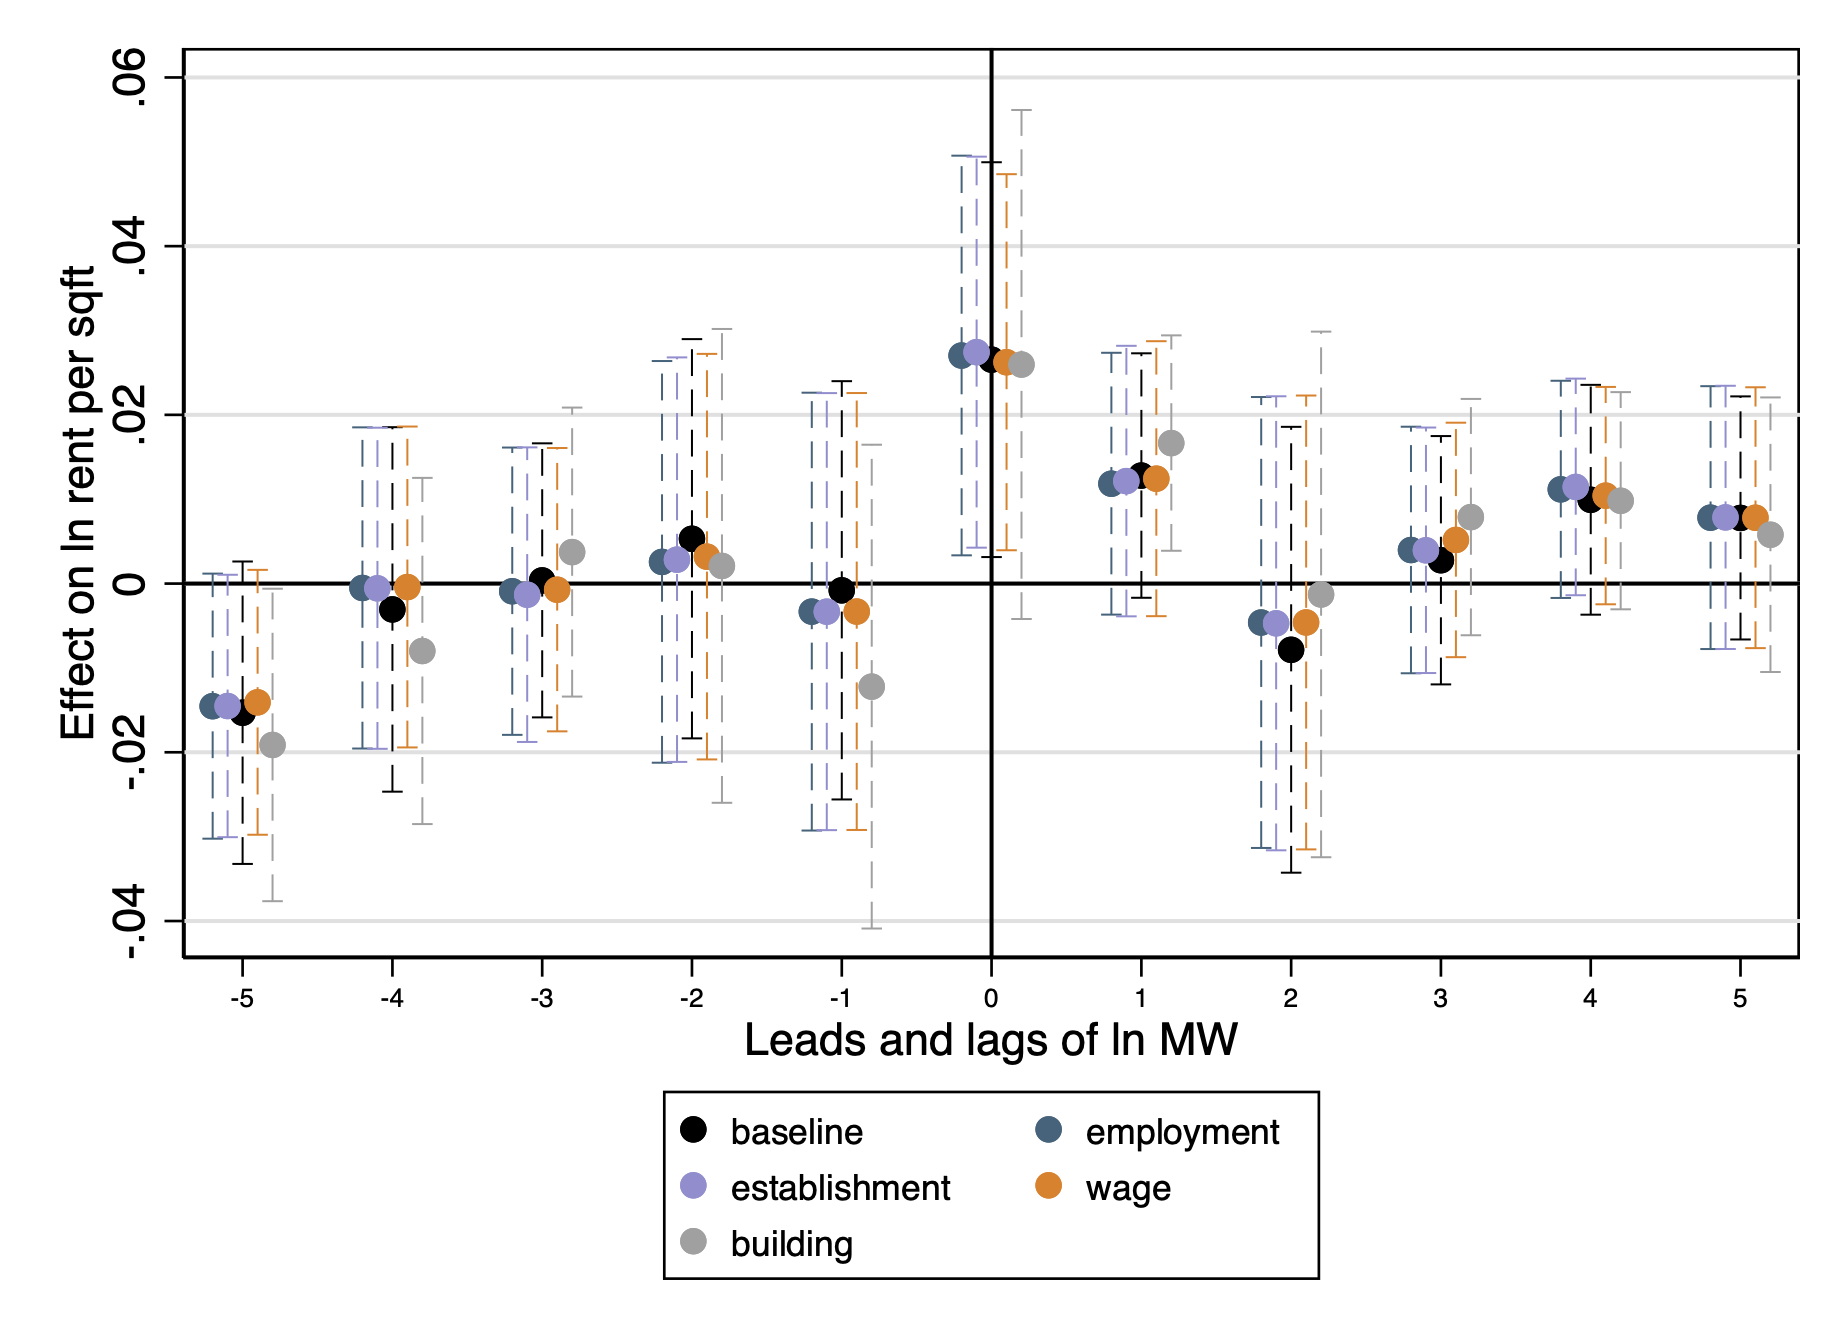
\includegraphics[width = 0.7\textwidth]{../analysis/first_differences/output/fd_models_control.png}
    \begin{minipage}{.95\textwidth} \footnotesize
		\vspace{2mm} 
		\textit{Notes}: The figure show estimates for $\hat{\beta}_{r}$ obtained from 
		\autoref{eq:leads_lags} when progressively adding time-varying controls for local shocks. 
		The \textit{baseline} series plots coefficients taken from 
		\autoref{tab:dynamic_leads_lags_econshock}, column (1). The \textit{employment}, 
		\textit{establishment}, \textit{wage}, and \textit{building} series plot coefficients 
		from \autoref{tab:dynamic_leads_lags_econshock}, columns (2) to (5) respectively. 90 
		percent confidence intervals reported.  
	\end{minipage}
\end{figure}



\end{document}